In this section, we compare \gls{MLD} with two variants presented in \Cref{apdx:mld_details} : \gls{MLD Inpaint}, a naive approach without our proposed \textit{multi-time masked} \gls{SDE}, \gls{MLD Uni} a variant of our method using the same training scheme of \cite{bao2023transformer}. We also analyse the effect of the $d$ randomization parameter on \gls{MLD} performance through ablations study. 
\subsection{MLD and its variants}
\Cref{table:mld_variants_comparison} summarizes the different approaches adopted in each variant. All the considered models share the same deterministic autoencoders trained during the first stage. 

For fairness, our evaluation was done using the same configuration and code basis of \gls{MLD}. This includes: the autoencoder architectures and latent space size (similar to \Cref{sec:experiments}), the same score network (\Cref{fig:score_net}) is used across experiments, with \gls{MLD Inpaint} using the same architecture with one time dimension instead of the multi-time vector.
In all the variants, the joint and conditional generation are conducted using the same reverse sampling schedule described in \Cref{sec:repaint_sche}. 


\begin{table}[h]
\caption{\gls{MLD} and its variants ablation study}
\centering
\begin{tabular}{c|c|c|c}
\toprule
Model & Multi-time diffusion & Training & Conditional and joint generation
 \\
\midrule 
\gls{MLD Inpaint} & x & \Cref{elbo_diff_j} & \Cref{algo:MLD_inpaint_cond}  \\
\gls{MLD Uni} & \checkmark & \cite{bao2023transformer} & \Cref{algo:MLD_cond_gen}  \\
\gls{MLD} & \checkmark & \Cref{algo:MLD_training} & \Cref{algo:MLD_cond_gen}  \\
\bottomrule
\end{tabular}
\label{table:mld_variants_comparison}
\end{table}



\paragraph{Results}
In some cases, the \gls{MLD} variants can match the joint generation performance of \gls{MLD} but, overall, they are less efficient and have noticeable weaknesses: \gls{MLD Inpaint} under-performs in conditional generation when considering relatively complex modalities, \gls{MLD Uni} is not able to leverage the presence of multiple modalities to improve cross generation, especially for data-sets with a large number of modalities. On the other hand, \gls{MLD} is able to overcome all these limitations.


\paragraph{\mnist-\svhn.} 
In \Cref{coh_quality:ms_detailed_mld}, \gls{MLD} achieves the best results and dominates cross generation performance. We observe that \gls{MLD Inpaint} lacks coherence for \svhn to \mnist conditional generation, a results we expected by analysing the experiment in \Cref{fig:robust_exp}. \gls{MLD Uni}, despite the use of a multi-time diffusion process, under-performs our method, which indicates the effectiveness of our masked diffusion process in learning the conditional score network. Since all the models use the same deterministic autoencoders, the observed generative quality performance are relatively similar (See \Cref{fig:cond_joint_ms_detail} for qualitative results ).


\begin{table}[h]
\caption{Generation Coherence and Quality for MNIST-SVHN (M is for MNIST and S for SVHN ). The generation quality is measured in terms of FMD for MNIST and FID for SVHN.\newline}
 \label{coh_quality:ms_detailed_mld}
\centering
\resizebox{\textwidth}{!}{\begin{tabular}{c|c|cc|cc|cc}
\toprule
\multirow{2}{*}{ Models }  & \multicolumn{3}{c}{Coherence (\%$\uparrow$) } &   \multicolumn{4}{c}{Quality ($\downarrow$)} \\
    \cmidrule{2-8}
    & Joint &  M $\rightarrow$ S & S $\rightarrow$ M &
     Joint(M)  &  Joint(S) &M $\rightarrow$ S &  S $\rightarrow$ M  \\
    \midrule

    MLD-Inpaint & $\textbf{85.53}_{ \pm 0.22 } $& $\underline{81.76}_{\pm 0.23 }$ & $63.28_{\pm 1.16} $  &   $\textbf{3.85}_{ \pm 0.02}$ &
$ 60.86_{\pm 1.27}$&$59.86_{\pm1.18}$&
$\textbf{3.55}_{\pm 0.11} $ 
    \\
    MLD-Uni & $82.19_{ \pm 0.97} $& $79.31_{\pm 1.21 }$ & $\underline{72.78}_{\pm 1.81} $&  $4.1_{ \pm 0.17}$ &
$ 57.41_{\pm 1.43}$ &
$\underline{57.84}_{\pm1.57}$&
$4.84_{\pm 0.28} $

    \\
    MLD  & $\underline{85.22}_{ \pm 0.5}$ & $\textbf{83.79}_{\pm 0.62} $&$ \textbf{79.13}_{\pm 0.38}$ & $\underline{3.93}_{ \pm 0.12}$ &
    $\textbf{56.36}_{\pm1.63}$   &
    $\textbf{	57.2}_{\pm1.47}$  &
    $\underline{3.67}_{\pm 0.14} $ 
    \\
    \bottomrule
   
\end{tabular}}
\end{table}






\begin{figure}[h]
     \centering

\begin{subfigure}{0.25\textwidth}
         \centering
         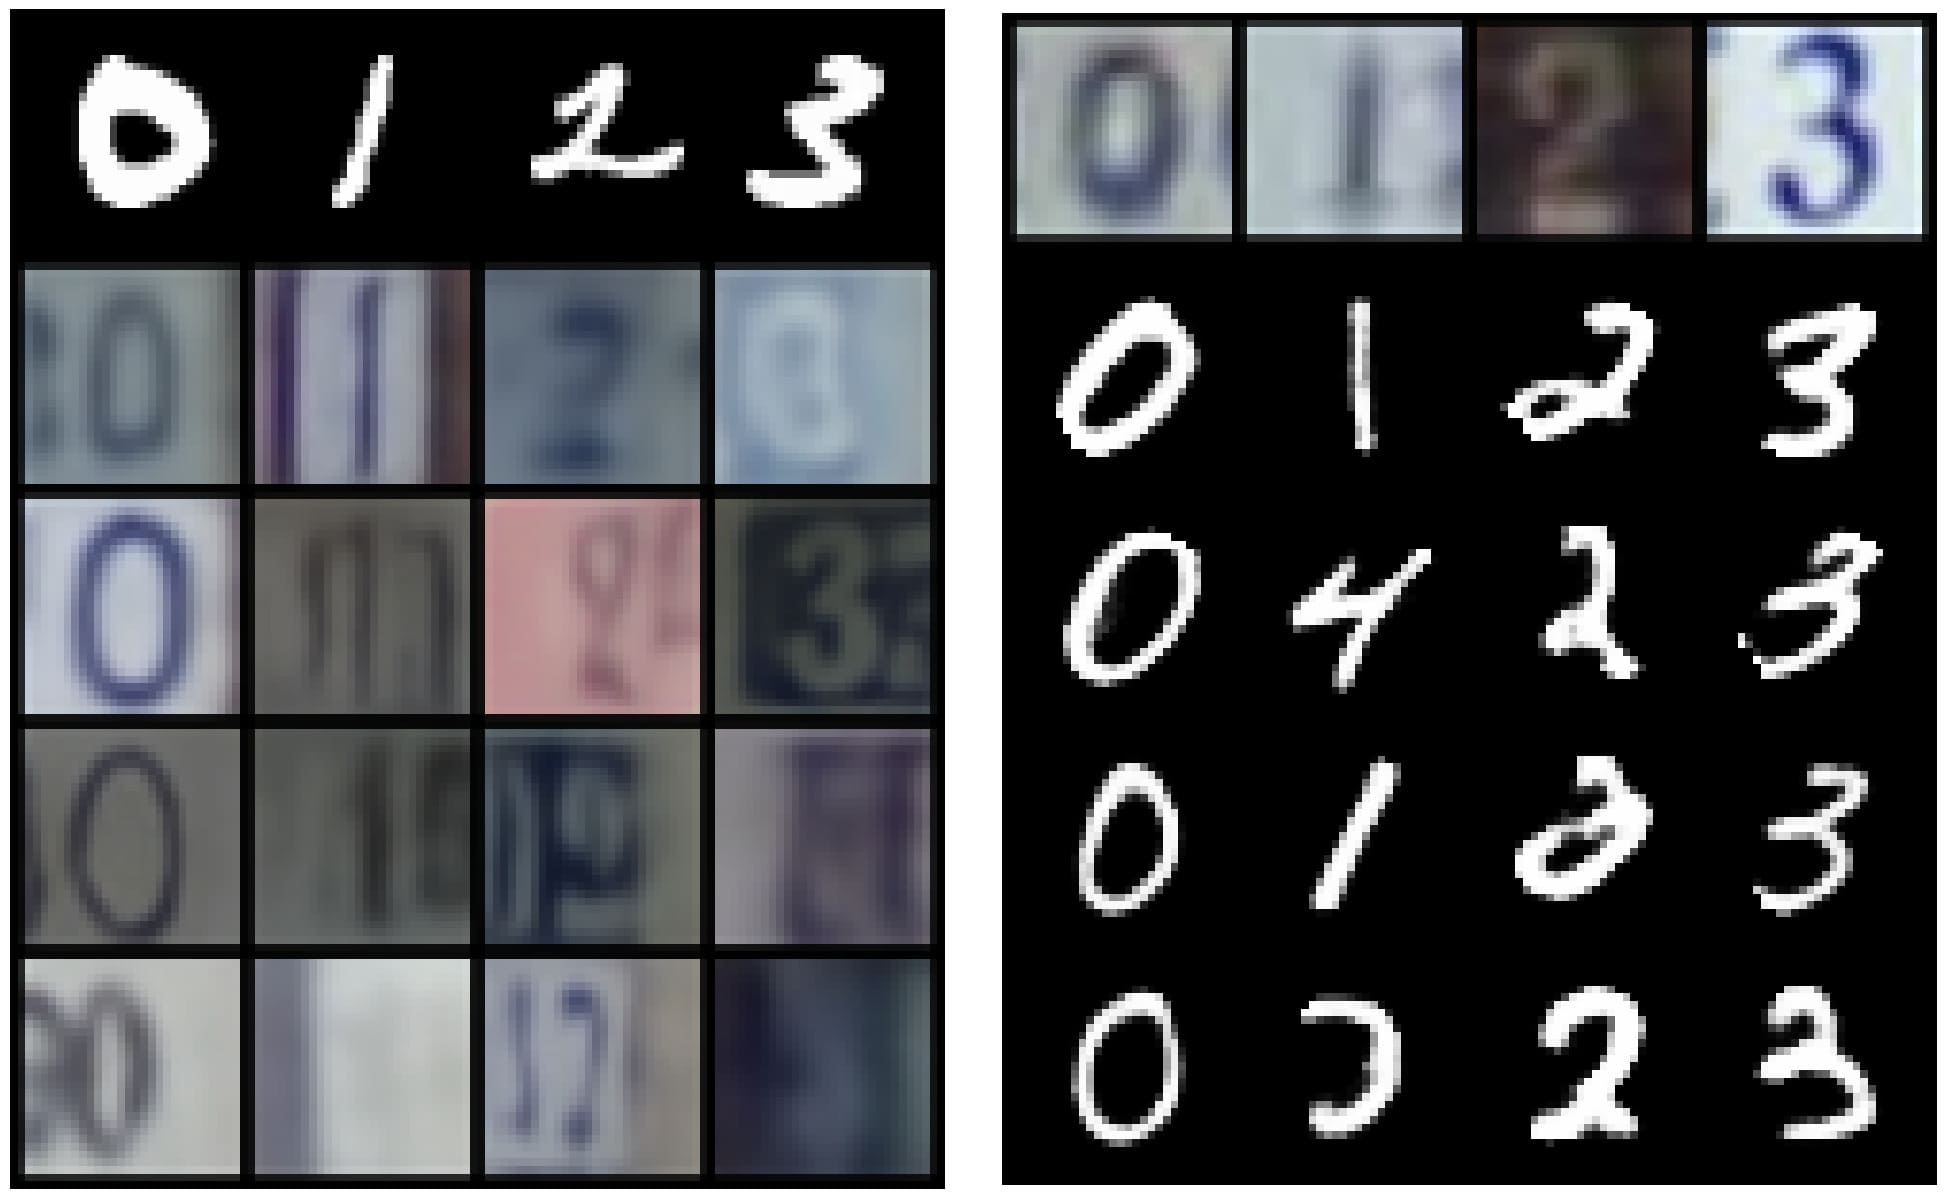
\includegraphics[width=\linewidth]{figures/datasets/ms/small_mld_MLD_inpaint_cond_mnist_svhn}
    \caption*{\gls{MLD Inpaint}}
    \end{subfigure}
\begin{subfigure}{0.25\textwidth}
         \centering
         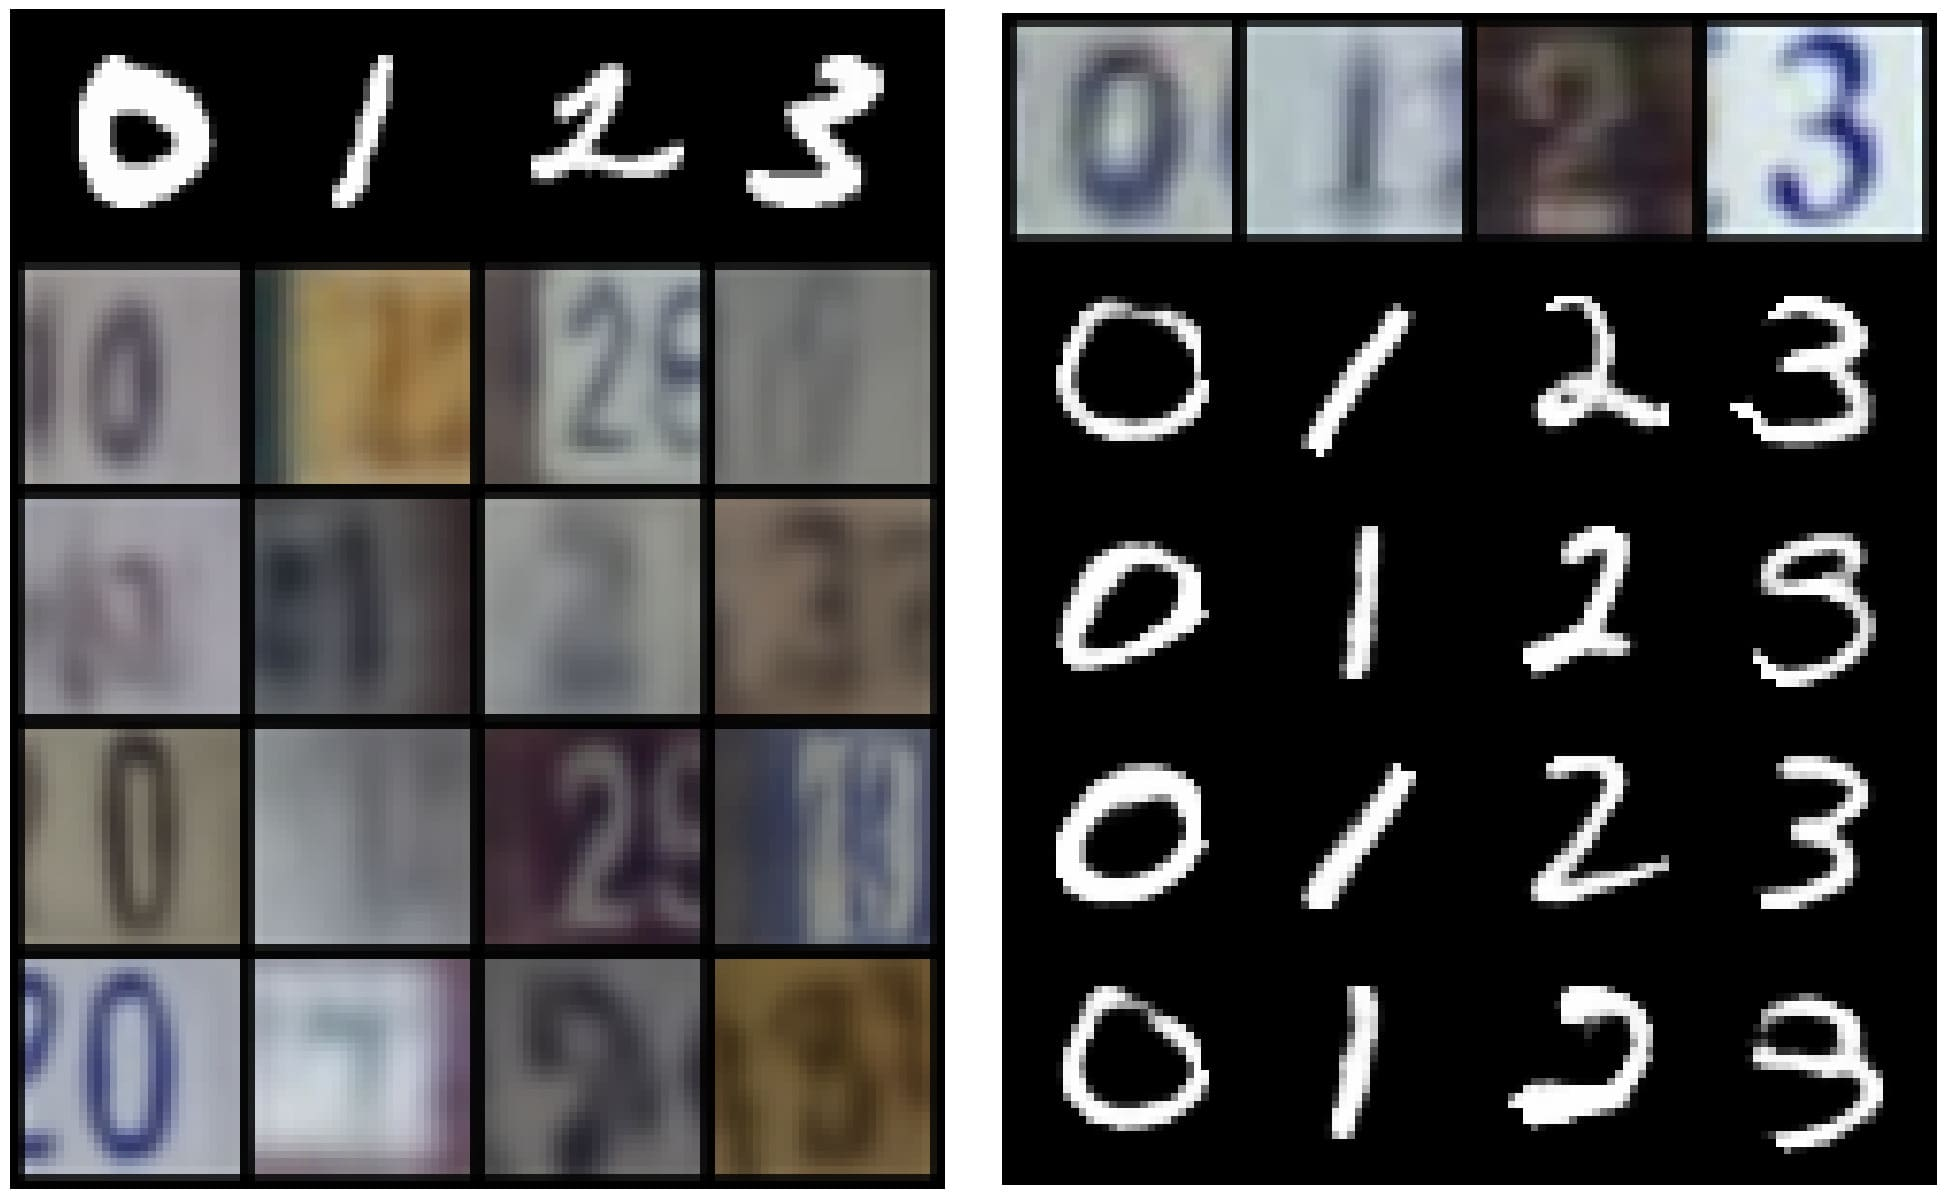
\includegraphics[width=\linewidth]{figures/datasets/ms/small_mld_MLD_uni_cond_mnist_svhn}
         \caption*{\gls{MLD Uni}}
\end{subfigure}
  \begin{subfigure}{0.25\textwidth}
         \centering
         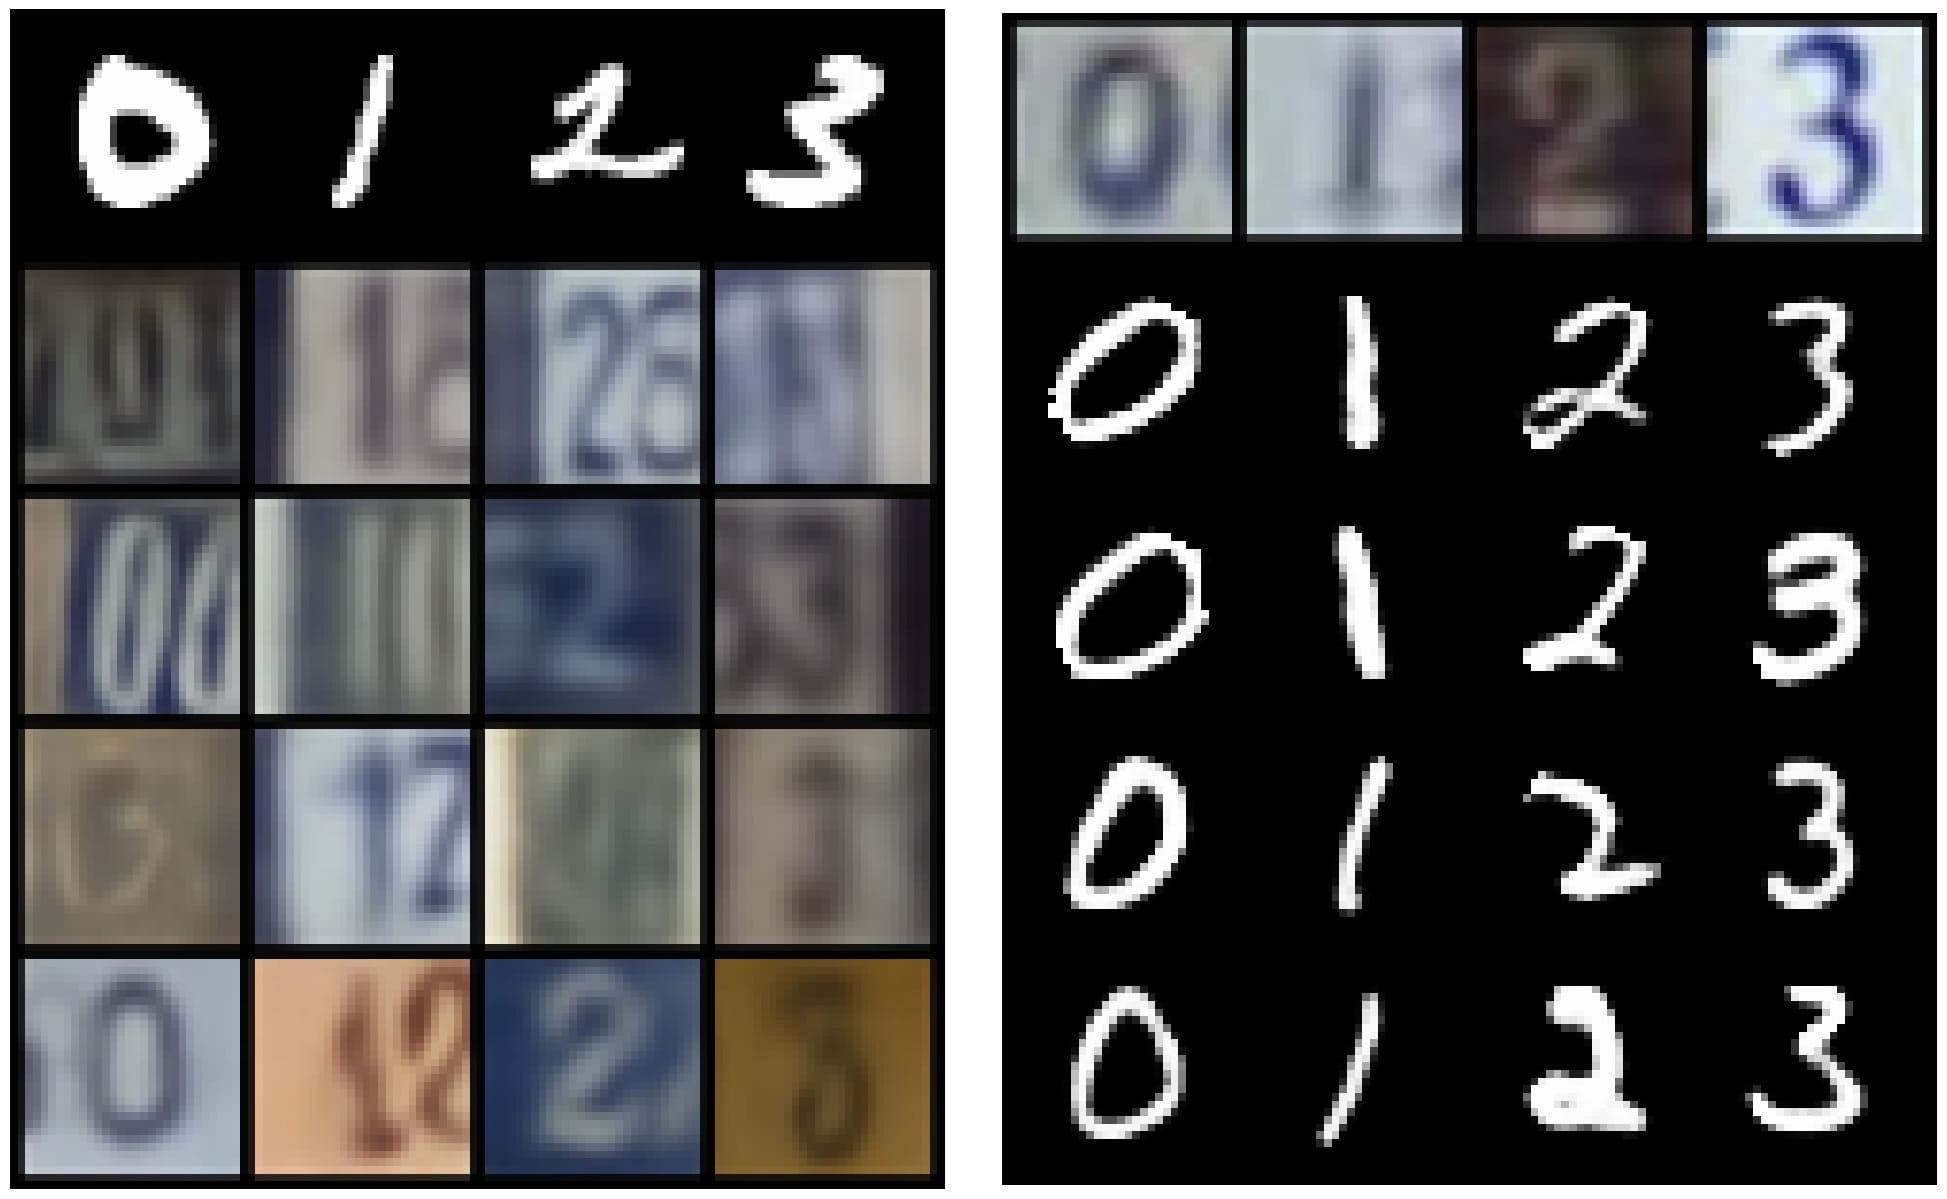
\includegraphics[page=1,width=\linewidth]{figures/datasets/ms/small_mld_MLD_cond_mnist_svhn}
         \caption*{\textbf{\gls{MLD}}}
     \end{subfigure}
\caption{Qualitative results for \textbf{\mnist-\svhn}. For each model we report: \mnist to \svhn conditional generation in the left,   \svhn to \mnist conditional generation in the right.}
        \label{fig:cond_joint_ms_detail}
\end{figure}







\paragraph{\mhd.} \Cref{coh:mhd_detailed_mld} shows the performance results for the \mhd data-set in terms of generative coherence.
\gls{MLD} achieves the best joint generation coherence and, along with \gls{MLD Uni}, they dominate the cross generation coherence. \gls{MLD Inpaint} shows a lack of coherence when conditioning on the sound modality alone, a predictable result since this is a more difficult configuration, as the sound modality is loosely correlated to other modalities. We also observe that \gls{MLD Inpaint} performs worse than the two other alternatives when conditioned on the trajectory modality, which is the smallest modality in terms of latent size. This indicates another limitation of the naive approach regarding coherent generation when handling different latent spaces sizes, a weakness our method \gls{MLD} overcomes. \Cref{qua:mhd_detailed_mld} presents the qualitative generative performance which are homogeneous across the variants with \gls{MLD}, achieving either the best or second best performance.



\begin{table}[H]
\centering
\caption{Generation Coherence (\%$\uparrow$) for \mhd  (Higher is better). Line above refers to the generated modality
while the observed modalities subset are presented below. \newline}
 \label{coh:mhd_detailed_mld}
\resizebox{\textwidth}{!}{\begin{tabular}{c|c|ccc|ccc|ccc}
\toprule
\multirow{2}{*}{ Models }  & \multirow{2}{*}{ Joint }
& \multicolumn{3}{c}{I (Image)}  & \multicolumn{3}{c}{T (Trajectory)}  & \multicolumn{3}{c}{S (Sound) } 
\\
\cmidrule{3-11}
    &&  T & S  & T,S  & I & S  & I,S & I & T & I,T \\
    \midrule

MLD-Inpaint  &  
$96.88_{ \pm 0.35 }$ &
    $63.9_{\pm 1.7 }$ & 
    $56.52 _{\pm 1.89 }$ &
     $ 95.83_{\pm 0.48}$ &
     
    $\underline{99.58}_{ \pm 0.1  }$  &
    $56.51 _{\pm  1.89 }$  &
    $\underline{99.89}_{\pm0.04}$ &  
    $95.81_{\pm0.25}$ &
    $56.51 _{\pm  1.89 }$  &
    $96.38_{\pm0.35}$   \\
    
MLD-Uni &  
  $\underline{97.69}_{ \pm 0.26 }$ &
    $\textbf{99.91}_{\pm 0.04 }$ &
    $\textbf{89.87}_{\pm 0.38 }$ & 
    $ \textbf{99.92}_{\pm 0.04}$ & 
    $\textbf{99.68}_{ \pm 0.1  }$  & 
    $\textbf{89.78}_{\pm  0.45 }$  & 
    $99.38_{\pm0.31}$ & 
    $\underline{97.54}_{\pm0.2}$ & 
    $\underline{97.65}_{\pm  0.41 }$ 
    & $\underline{97.79}_{\pm 0.41}$ 
    \\
 MLD &  
 $\textbf{98.34}_{ \pm 0.22 }$
 &
    $99.45_{\pm 0.09 }$ &
    $\underline{88.91}_{\pm 0.54 }$ & 
    $ \underline{99.88}_{\pm 0.04}$ & 
    
    $\underline{99.58}_{ \pm 0.03  }$  & 
    $\underline{88.92} _{\pm  0.53 }$  & 
    $\textbf{99.91}_{\pm0.02}$ &  
    
    $\textbf{97.63}_{\pm0.14}$ & 
    $\textbf{97.7} _{\pm  0.34 }$ 
    & $\textbf{98.01}_{\pm 0.21}$  \\
    \bottomrule
   
\end{tabular}}



\end{table}





\begin{table}[H]
\centering
\caption{Generation quality for \mhd . The metrics reported are \gls{FMD} for Image and Trajectory modalities and \gls{FAD} for the sound modalities (Lower is better).  \newline}
 \label{qua:mhd_detailed_mld}
\resizebox{\textwidth}{!}{\begin{tabular}{c|cccc|cccc|cccc}
\toprule
\multirow{2}{*}{ Models }   
& \multicolumn{4}{c}{I (Image)}  & \multicolumn{4}{c}{T (Trajectory)}  & \multicolumn{4}{c}{S (Sound) } 
\\
\cmidrule{2-13}
   & Joint & T & S  & T,S  &  Joint & I & S  & I,S & Joint & I & T & I,T   \\
    \midrule
      MLD-Inpaint &   
    $5.35_{ \pm 1.35 }$   &
    $6.23_{ \pm 1.13 }$ &
    $\underline{4.76}_{ \pm 0.68 }$  &
    $3.53_{ \pm 0.36 }$  &
   
    
    $\textbf{1.59}_{ \pm 0.12}$   & 
    $\textbf{0.6}_{ \pm 0.05}$ &
    $\textbf{1.81}_{ \pm 0.13 }$  &
    $\textbf{0.54}_{ \pm 0.06 }$  &
 
    
    $2.41_{ \pm 0.07}$ &
    $2.5_{ \pm 0.04}$ &
    $2.52_{ \pm 0.02 }$  &
    $2.49_{ \pm 0.05 }$  
   
    \\
    MLD-Uni &   
     $\textbf{7.91}_{ \pm 2.2 }$   &
    $\textbf{1.65}_{ \pm 0.33 }$ &
    $6.29_{ \pm 1.38 }$  &
    $\underline{3.06}_{ \pm 0.54 }$  &
   
    
    $\underline{2.53}_{ \pm 0.5}$   & 
    $1.18_{ \pm 0.26}$ &
    $3.18_{ \pm 0.77 }$  &
    $2.84_{ \pm 1.14 }$  
    
    
    & $\textbf{2.11}_{ \pm 0.08 }$
    & $\textbf{2.25}_{ \pm 0.05 }$ 
     & $\textbf{2.1}_{ \pm 0.0 }$ 
       & $\textbf{	2.15}_{ \pm 0.01 }$ 
       
      \\
    MLD &   
    $\underline{7.98}_{ \pm 1.41 }$ &
    $\underline{1.7}_{ \pm 0.14 }$ &
    $\textbf{4.54}_{ \pm 0.45 }$ & 
    $\textbf{1.84}_{ \pm 0.27 }$  

    
    & $3.18_{ \pm 0.18 }$ 
      & $\underline{0.83}_{ \pm 0.03 }$ 
     & $\underline{2.07}_{ \pm 0.26 }$ 
       & $\underline{0.6}_{ \pm 0.05}$ 
       


        & $ \underline{2.39}_{ \pm 0.1 } $
        & $\underline{2.31}_{ \pm 0.07 }$ 
     & $\underline{2.33}_{ \pm 0.11 }$ 
       & $\underline{	2.29}_{ \pm 0.06 }$ 
       
       \\

    \bottomrule
   
\end{tabular}}

\end{table}









\paragraph{\polymnist.} In \Cref{fig:res_mmnist_mld}, we remark the superiority of \gls{MLD} in both generative coherence and quality. {MLD-Uni} is not able to leverage the presence of a large number of modalities in conditional generation coherence. Interestingly, an increase in the number of input modalities impacts negatively the performance of \gls{MLD Uni}.

\begin{figure} [h]
     \centering
    \begin{subfigure}{0.25\textwidth}
     \begin{subfigure}{1\textwidth}
         \centering
         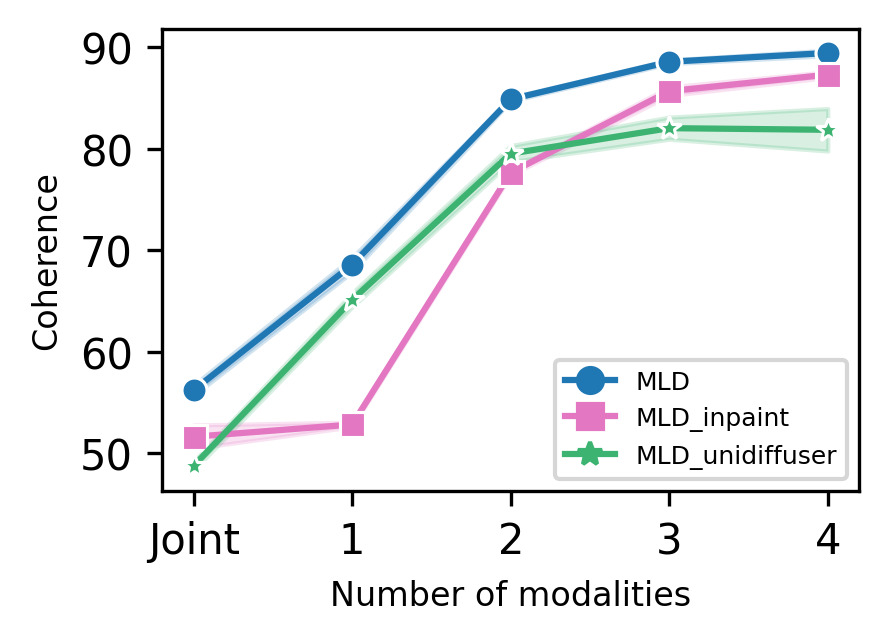
\includegraphics[page=1,width=\linewidth]{figures/datasets/mmnist/quant/mld_mmnist_plot_coh_avg}
     \end{subfigure}
     \begin{subfigure}{1\textwidth}
         \centering
         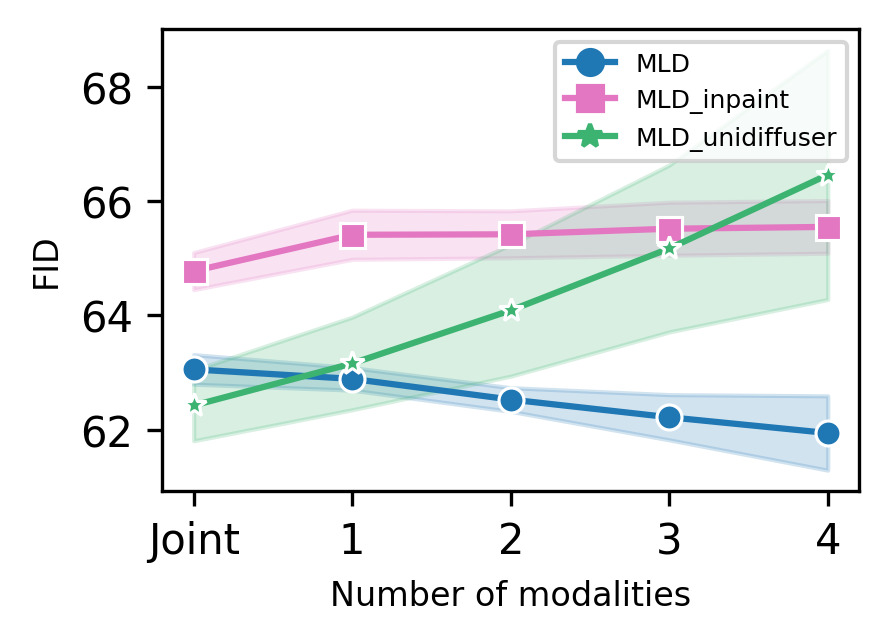
\includegraphics[width=\linewidth]{figures/datasets/mmnist/quant/mld_var_mmnist_plot_fid_avg}
         
     \end{subfigure}
\label{mmnist_quantitavie_mld}
\end{subfigure}
\begin{subfigure}{0.74\textwidth}
    \centering 
      \begin{subfigure}{0.29\textwidth}
         \centering
         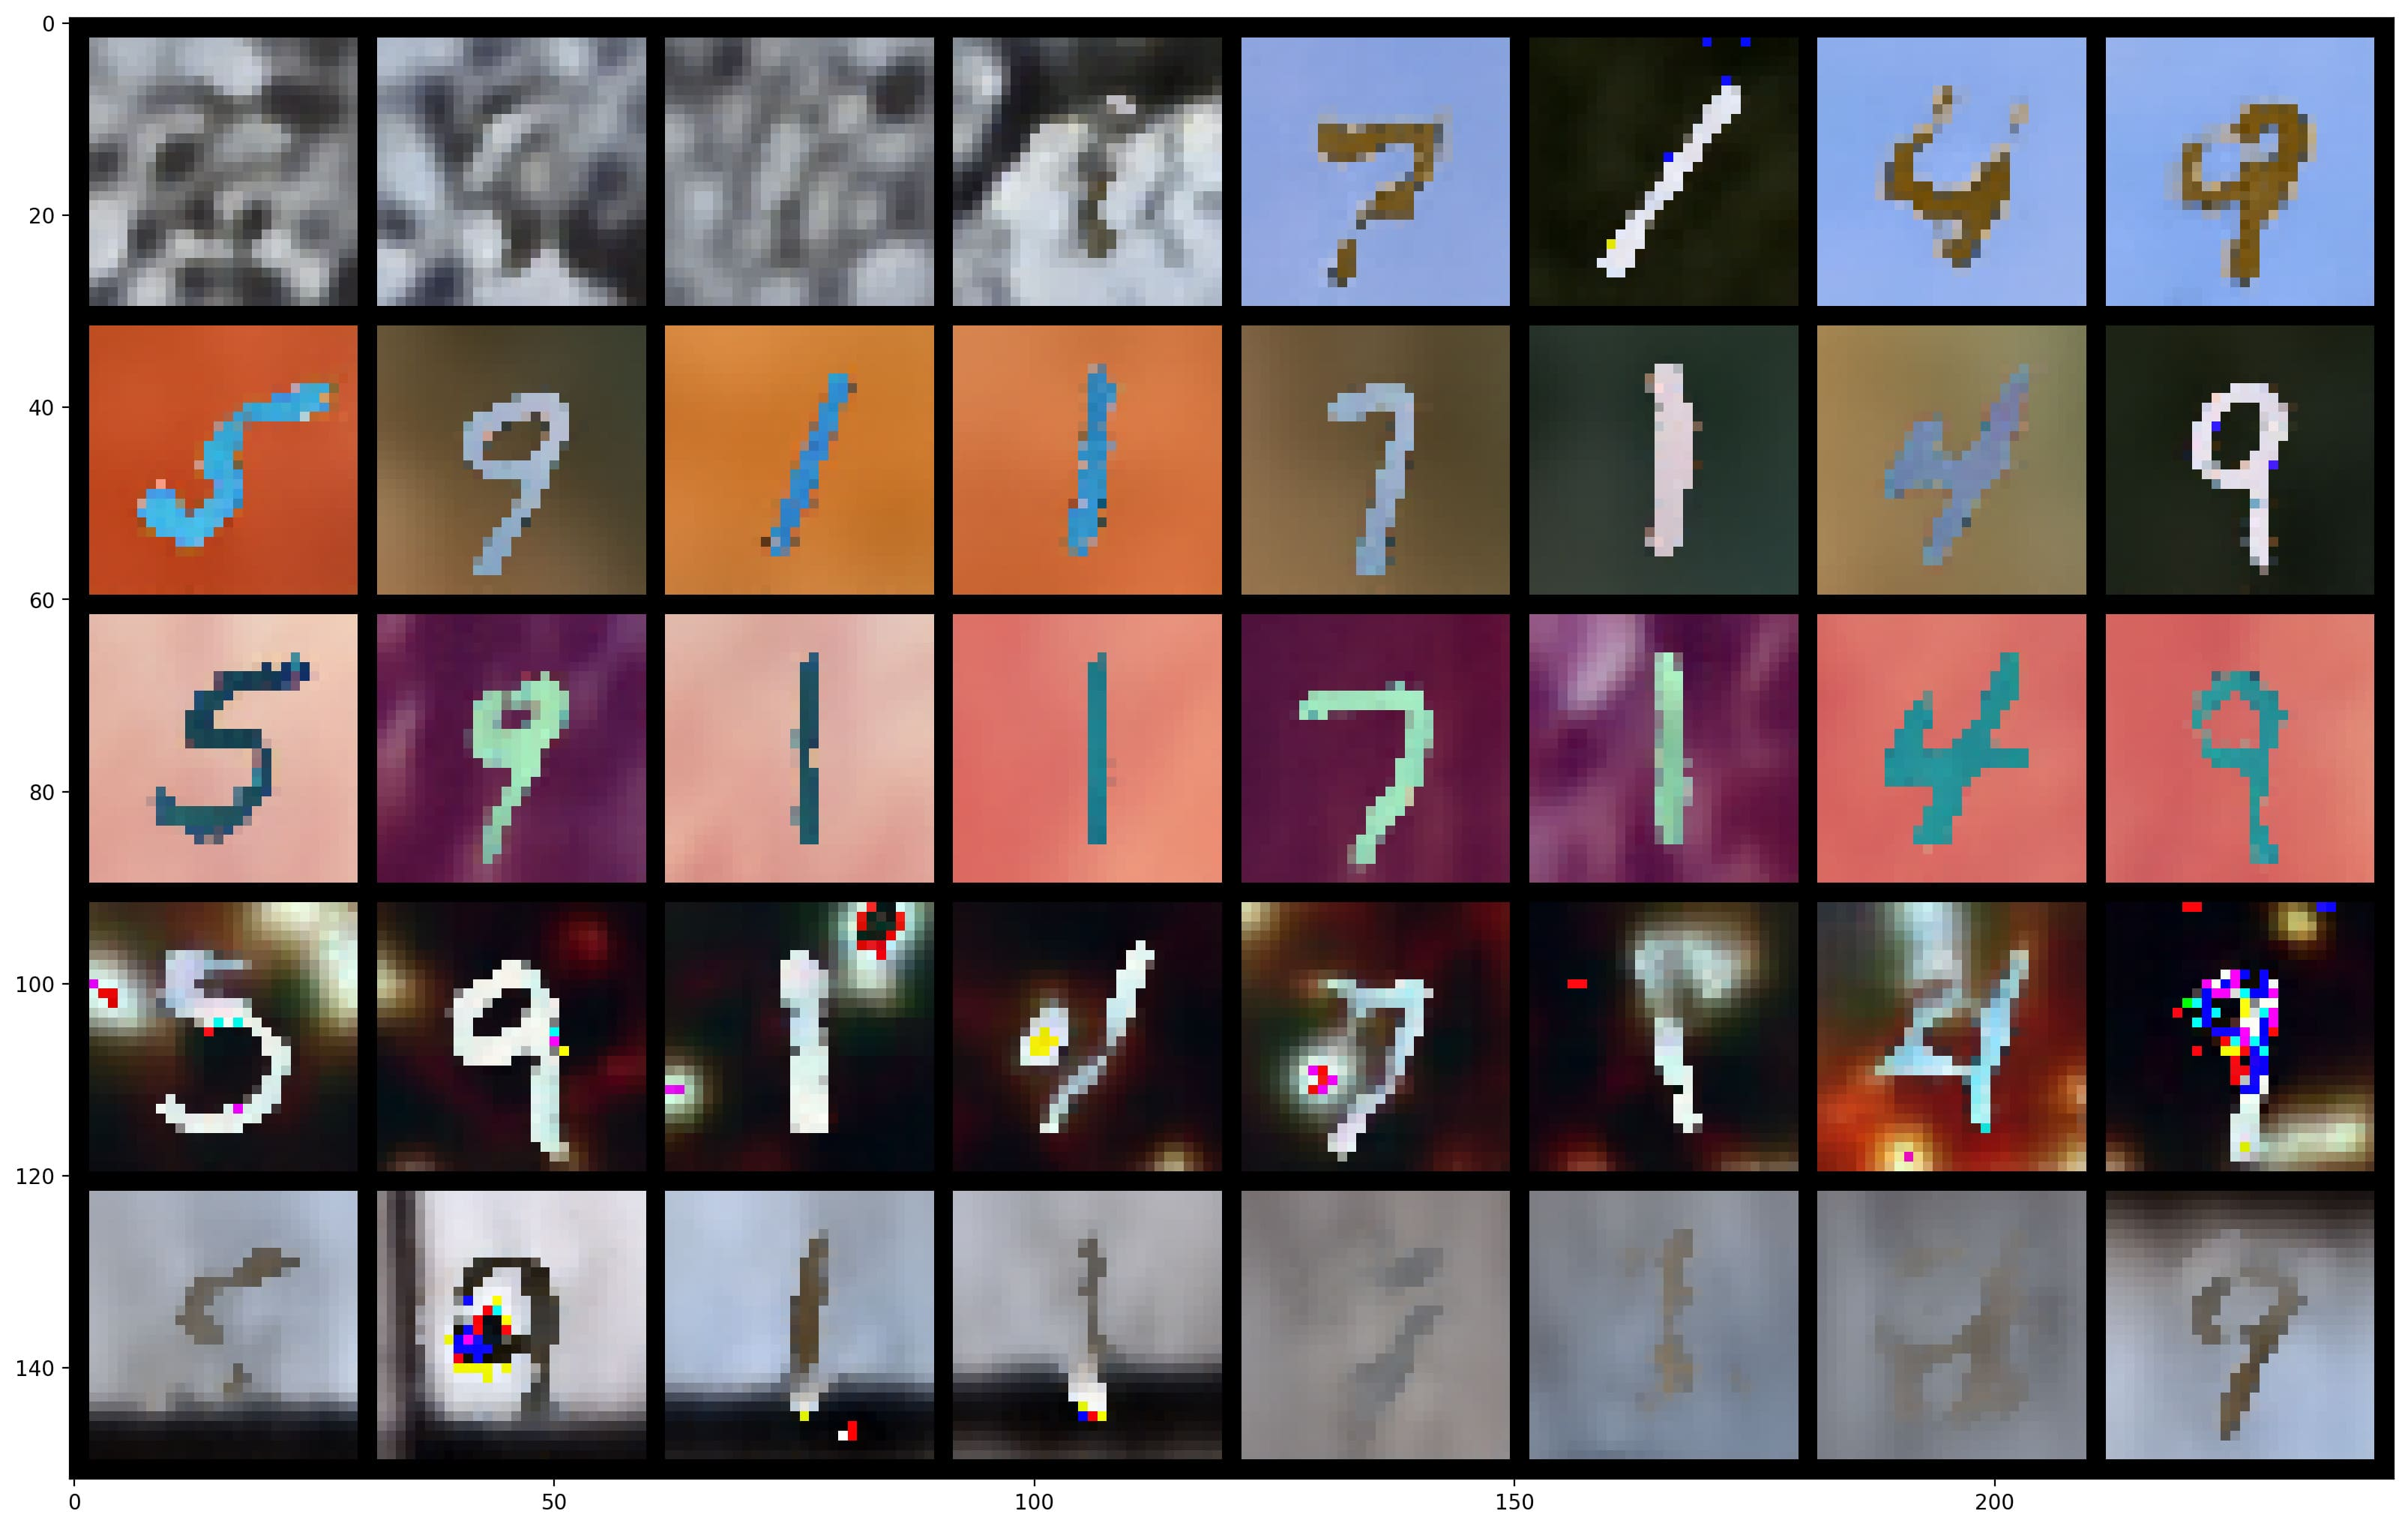
\includegraphics[width=\linewidth]{figures/datasets/mmnist/quali/MLD_inpaint_sampling}
         \caption*{\gls{MLD Inpaint}}
     \end{subfigure}
        \begin{subfigure}{0.29\textwidth}
         \centering
         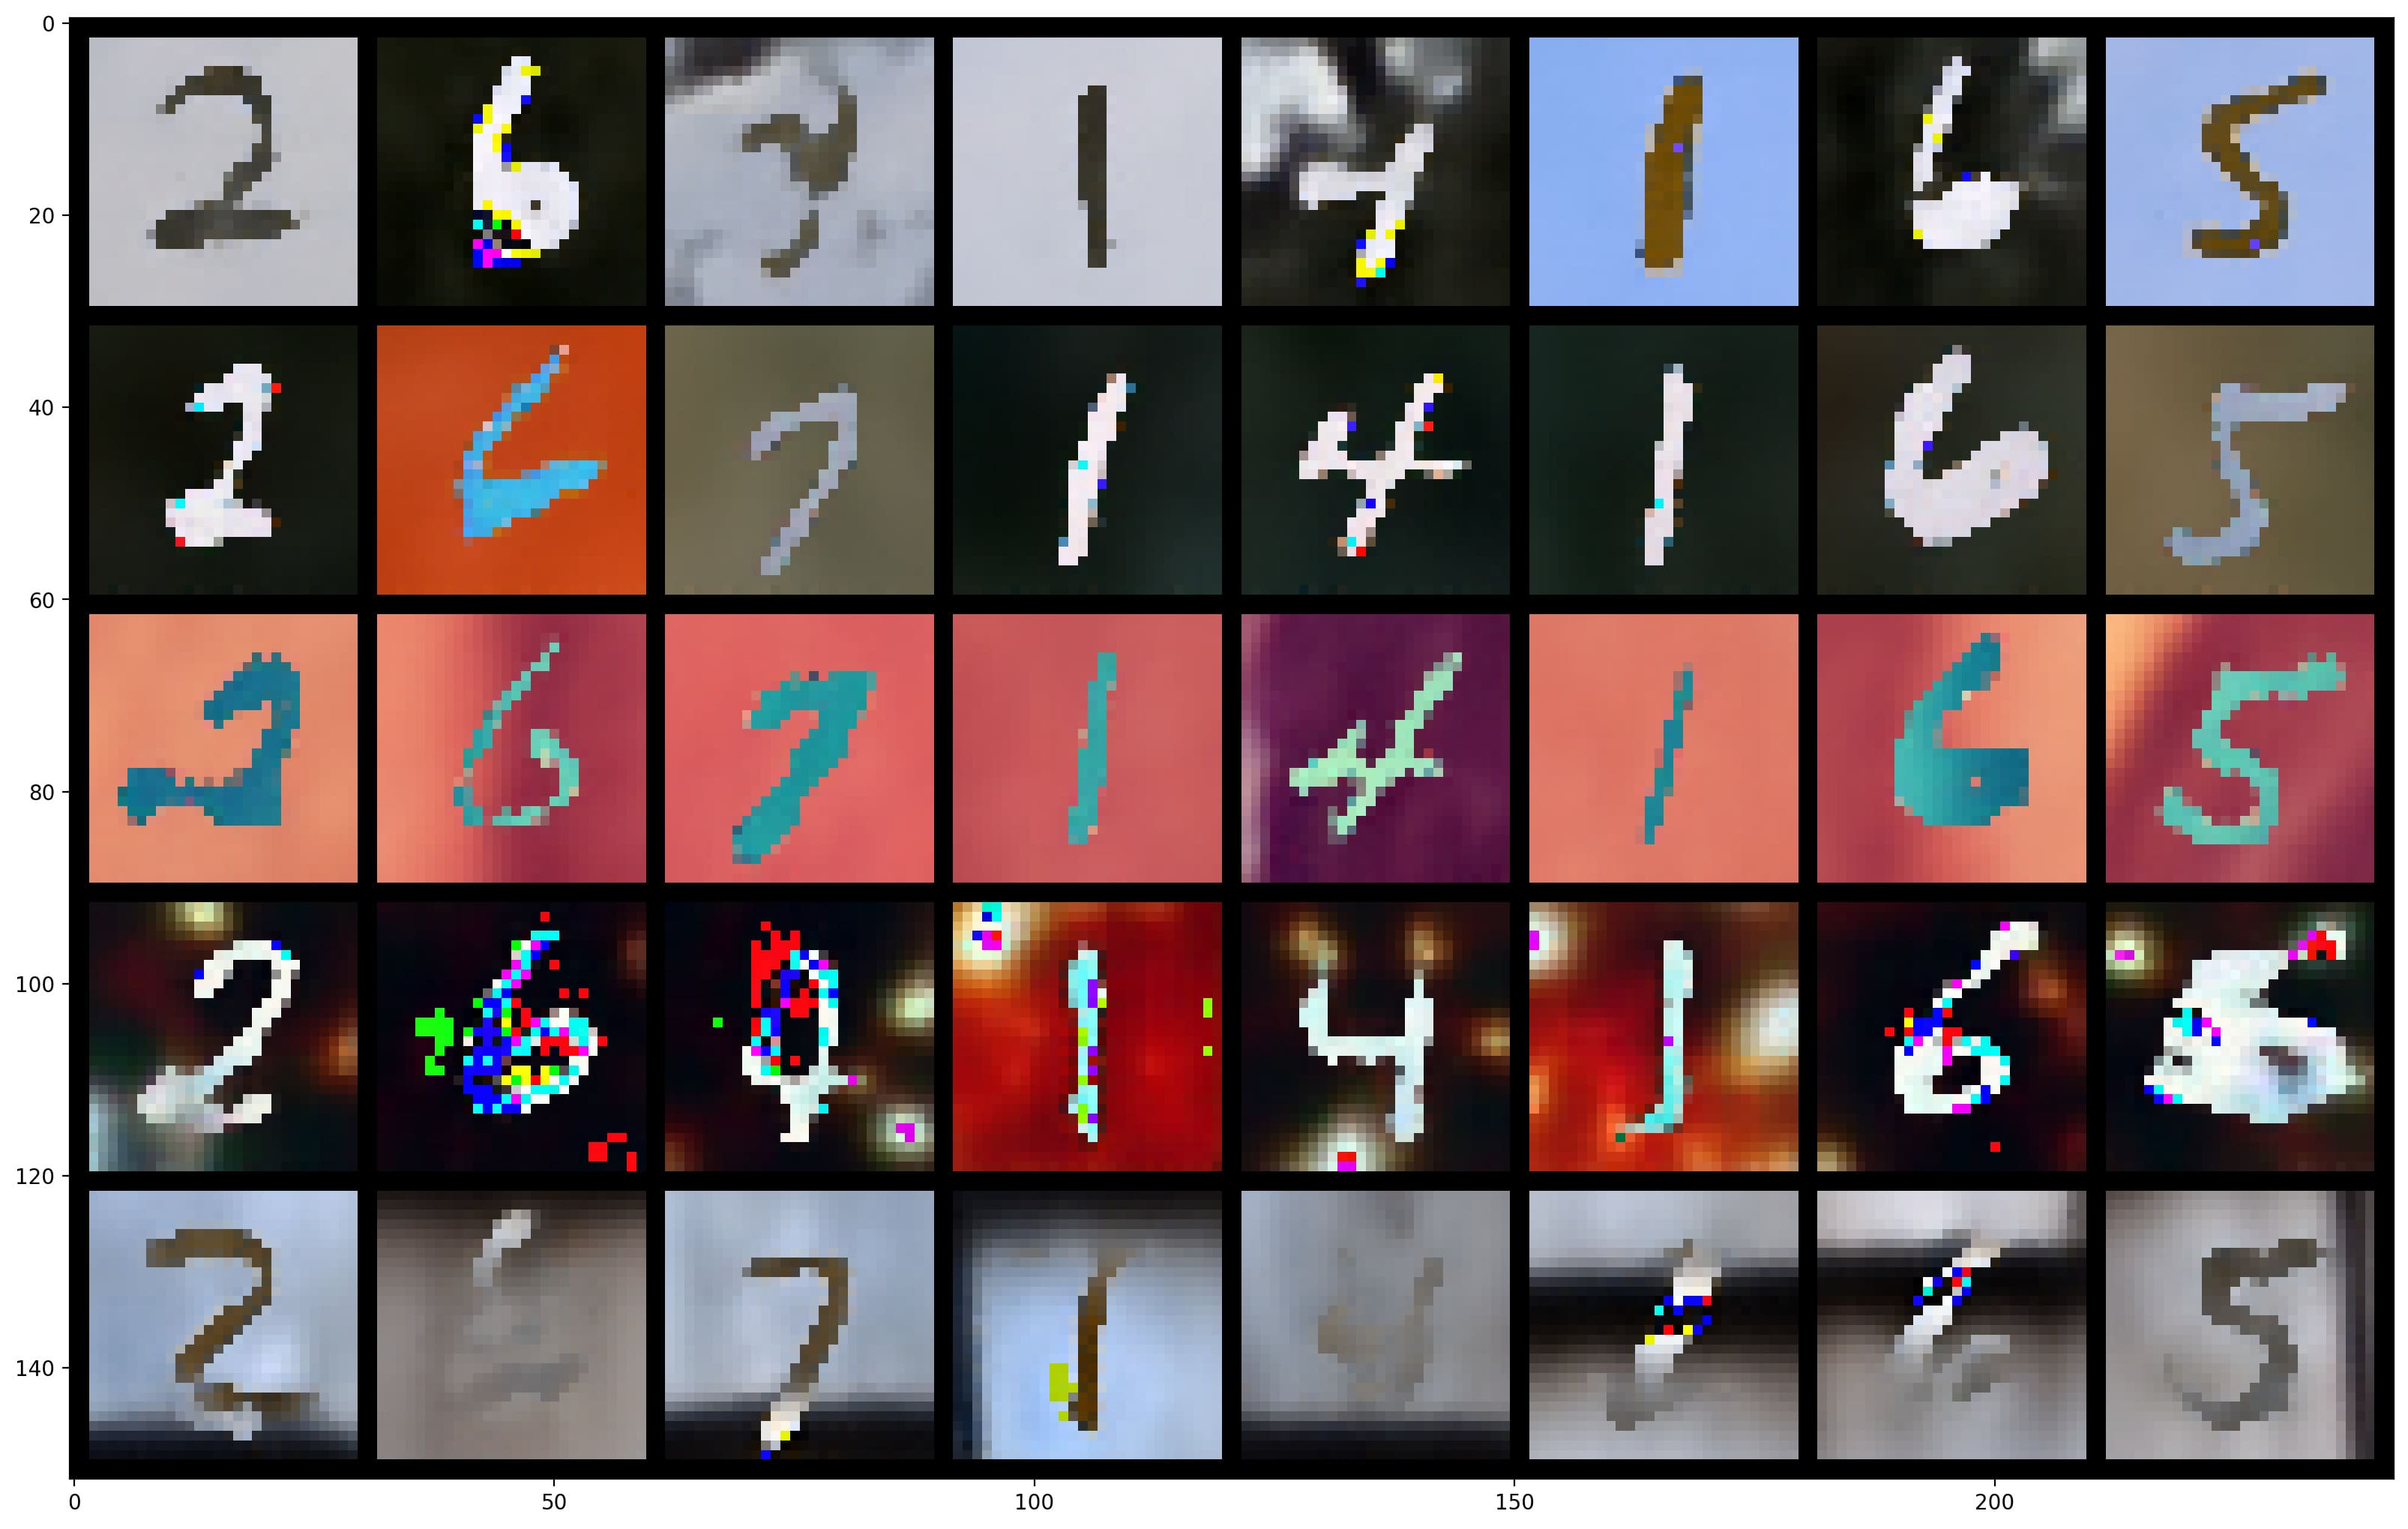
\includegraphics[width=\linewidth]{figures/datasets/mmnist/quali/MLD_uni_sampling}
         \caption*{\gls{MLD Uni}}
   
     \end{subfigure}
    
  \begin{subfigure}{0.29\textwidth}
         \centering
         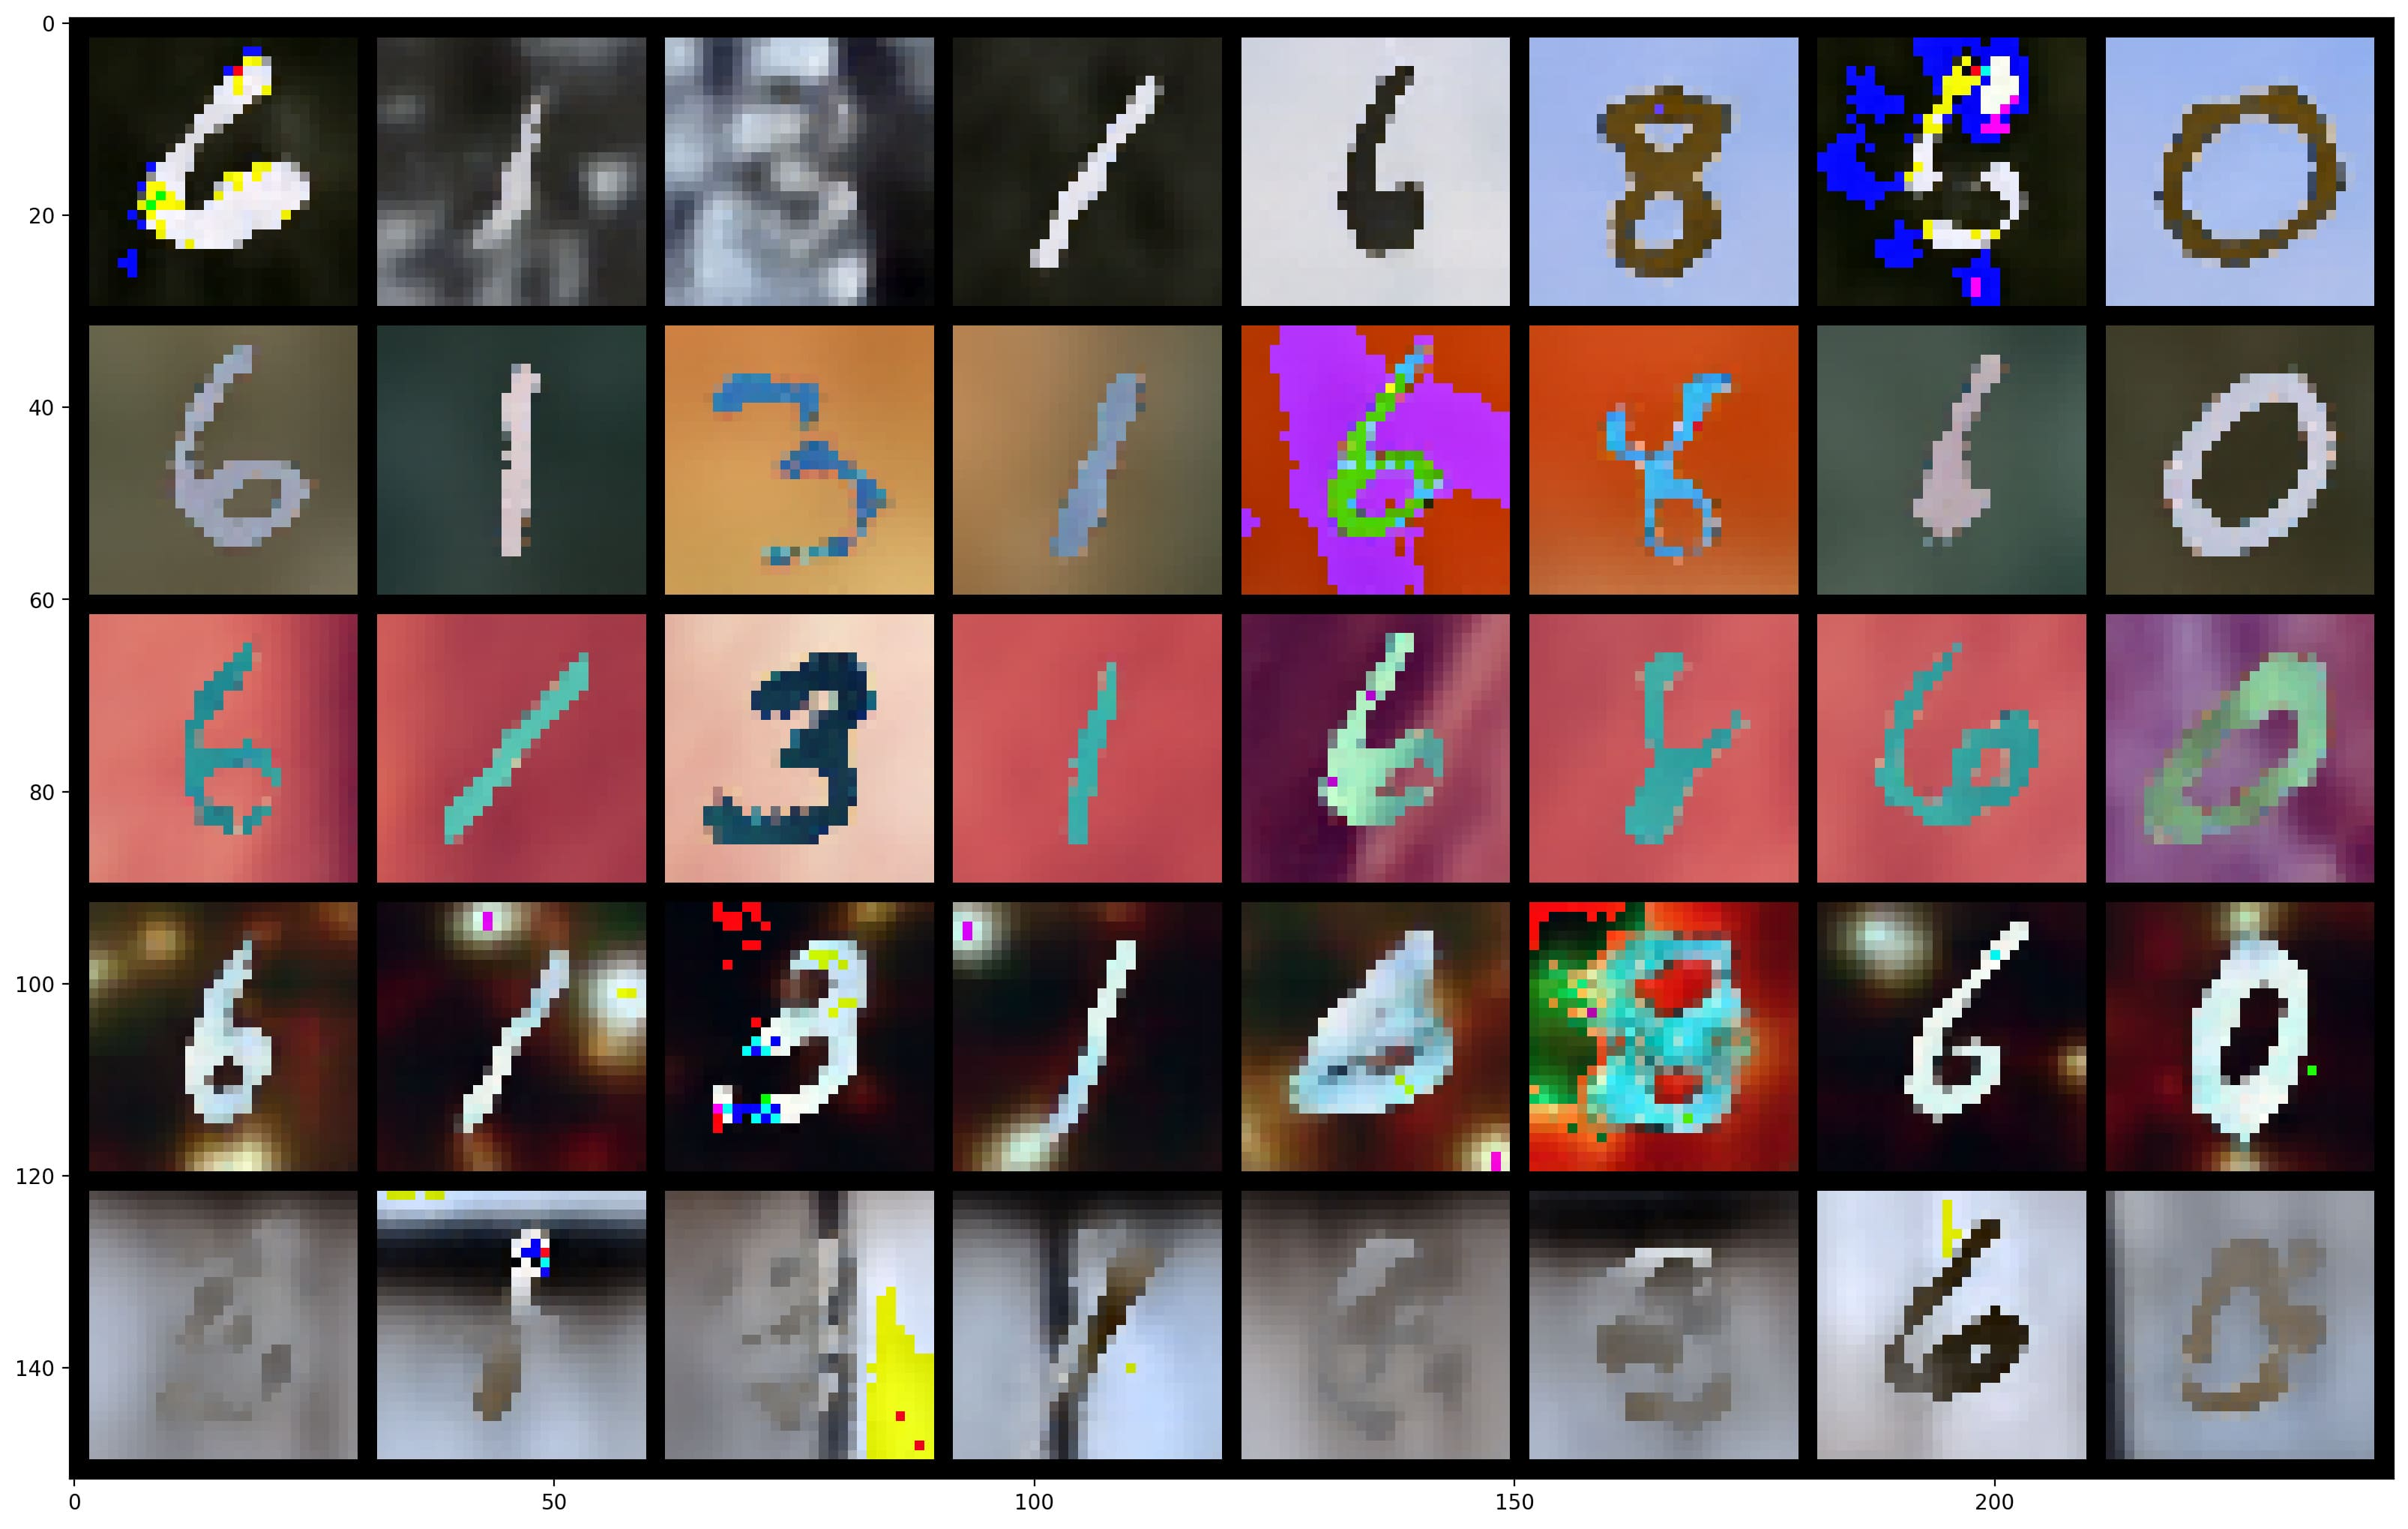
\includegraphics[page=1,width=\linewidth]{figures/datasets/mmnist/quali/MLD_sampling}
         \caption*{\textbf{\gls{MLD} }}
       
     \end{subfigure}
       \label{qual_mmnist_mld}
\end{subfigure}
        \caption{Results for \textbf{\polymnist} data-set. \textit{Left}: a comparison of the generative coherence (\% $\uparrow$) and quality in terms of \gls{FID} ($\downarrow$)) as a function of the number of modality input. We report the average performance following the leave-one-out strategy (see \Cref{apdx:dataset_eval}).  \textit{Right}: are qualitative results for the joint generation of the 5 modalities.   }
        \label{fig:res_mmnist_mld}
\end{figure}

\paragraph{\cub.} \Cref{cap_image_cub_mld} shows qualitative results for caption to image conditional generation. All the variants are based on the same first stage autoencoders, and the generative performance in terms of quality are comparable.


\begin{figure}[h]
     \centering
     \begin{subfigure}{0.19\textwidth}
         \centering
         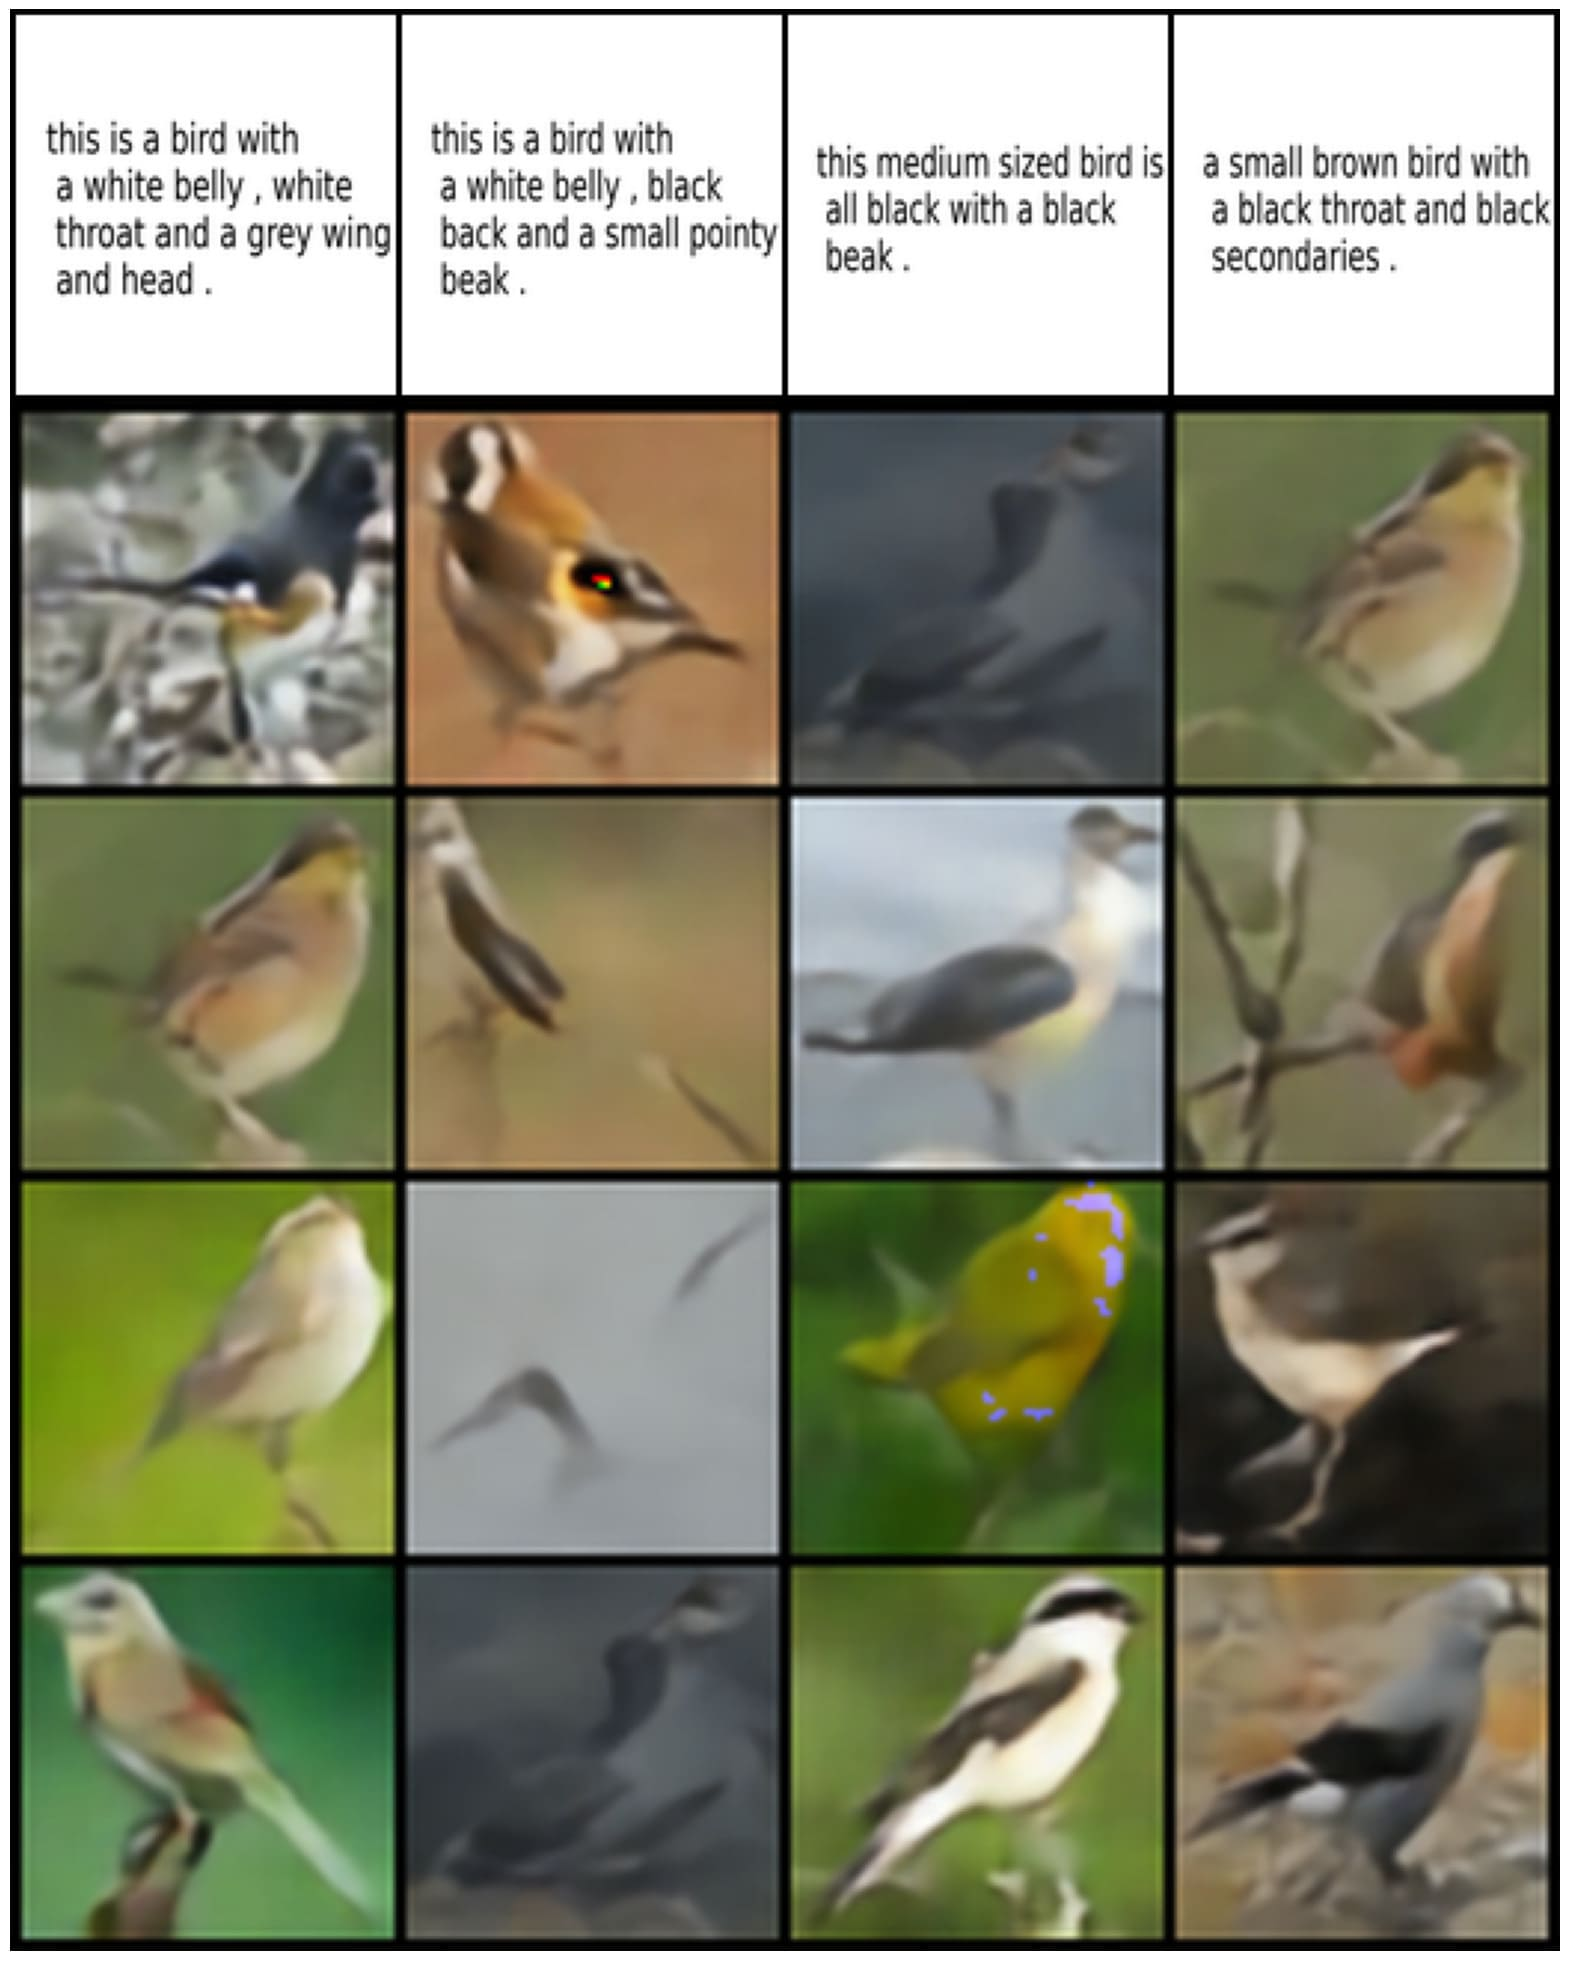
\includegraphics[width=\linewidth]{figures/datasets/cub/MLD_inpaint_cond_text_image_mld_var}
         \caption*{\gls{MLD Inpaint}} 
     \end{subfigure}
       \begin{subfigure}{0.19\textwidth}
         \centering
         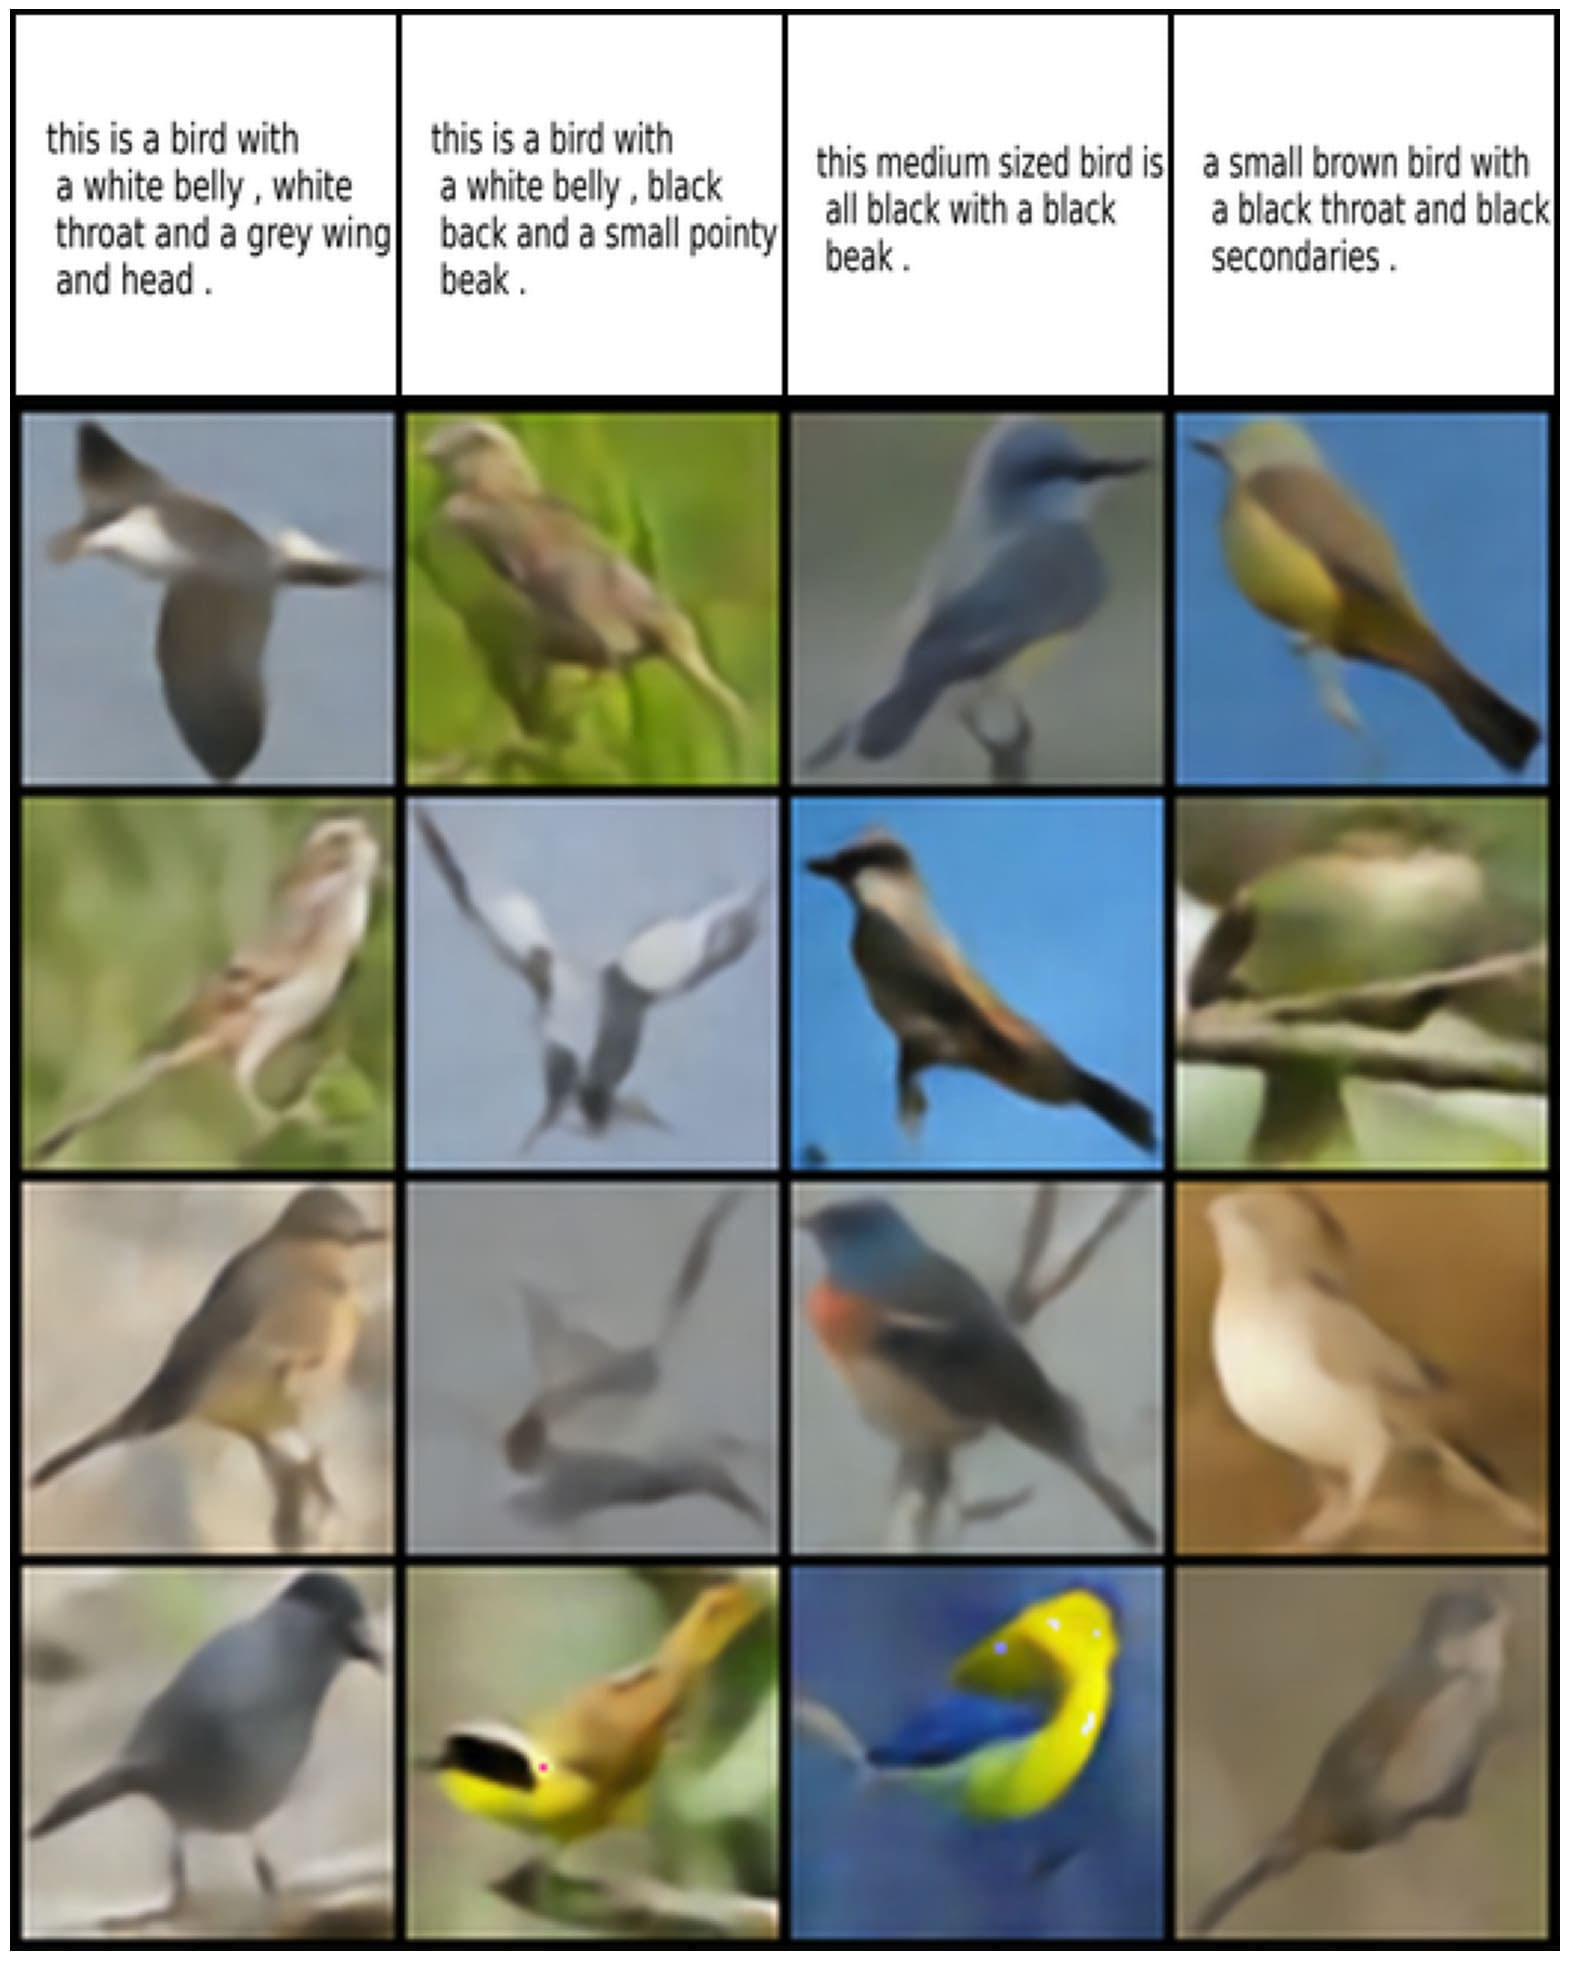
\includegraphics[width=\linewidth]{figures/datasets/cub/MLD_uni_cond_text_image_mld_var}
         \caption*{\gls{MLD Uni}}
     \end{subfigure}
  \begin{subfigure}{0.19\textwidth}
         \centering
         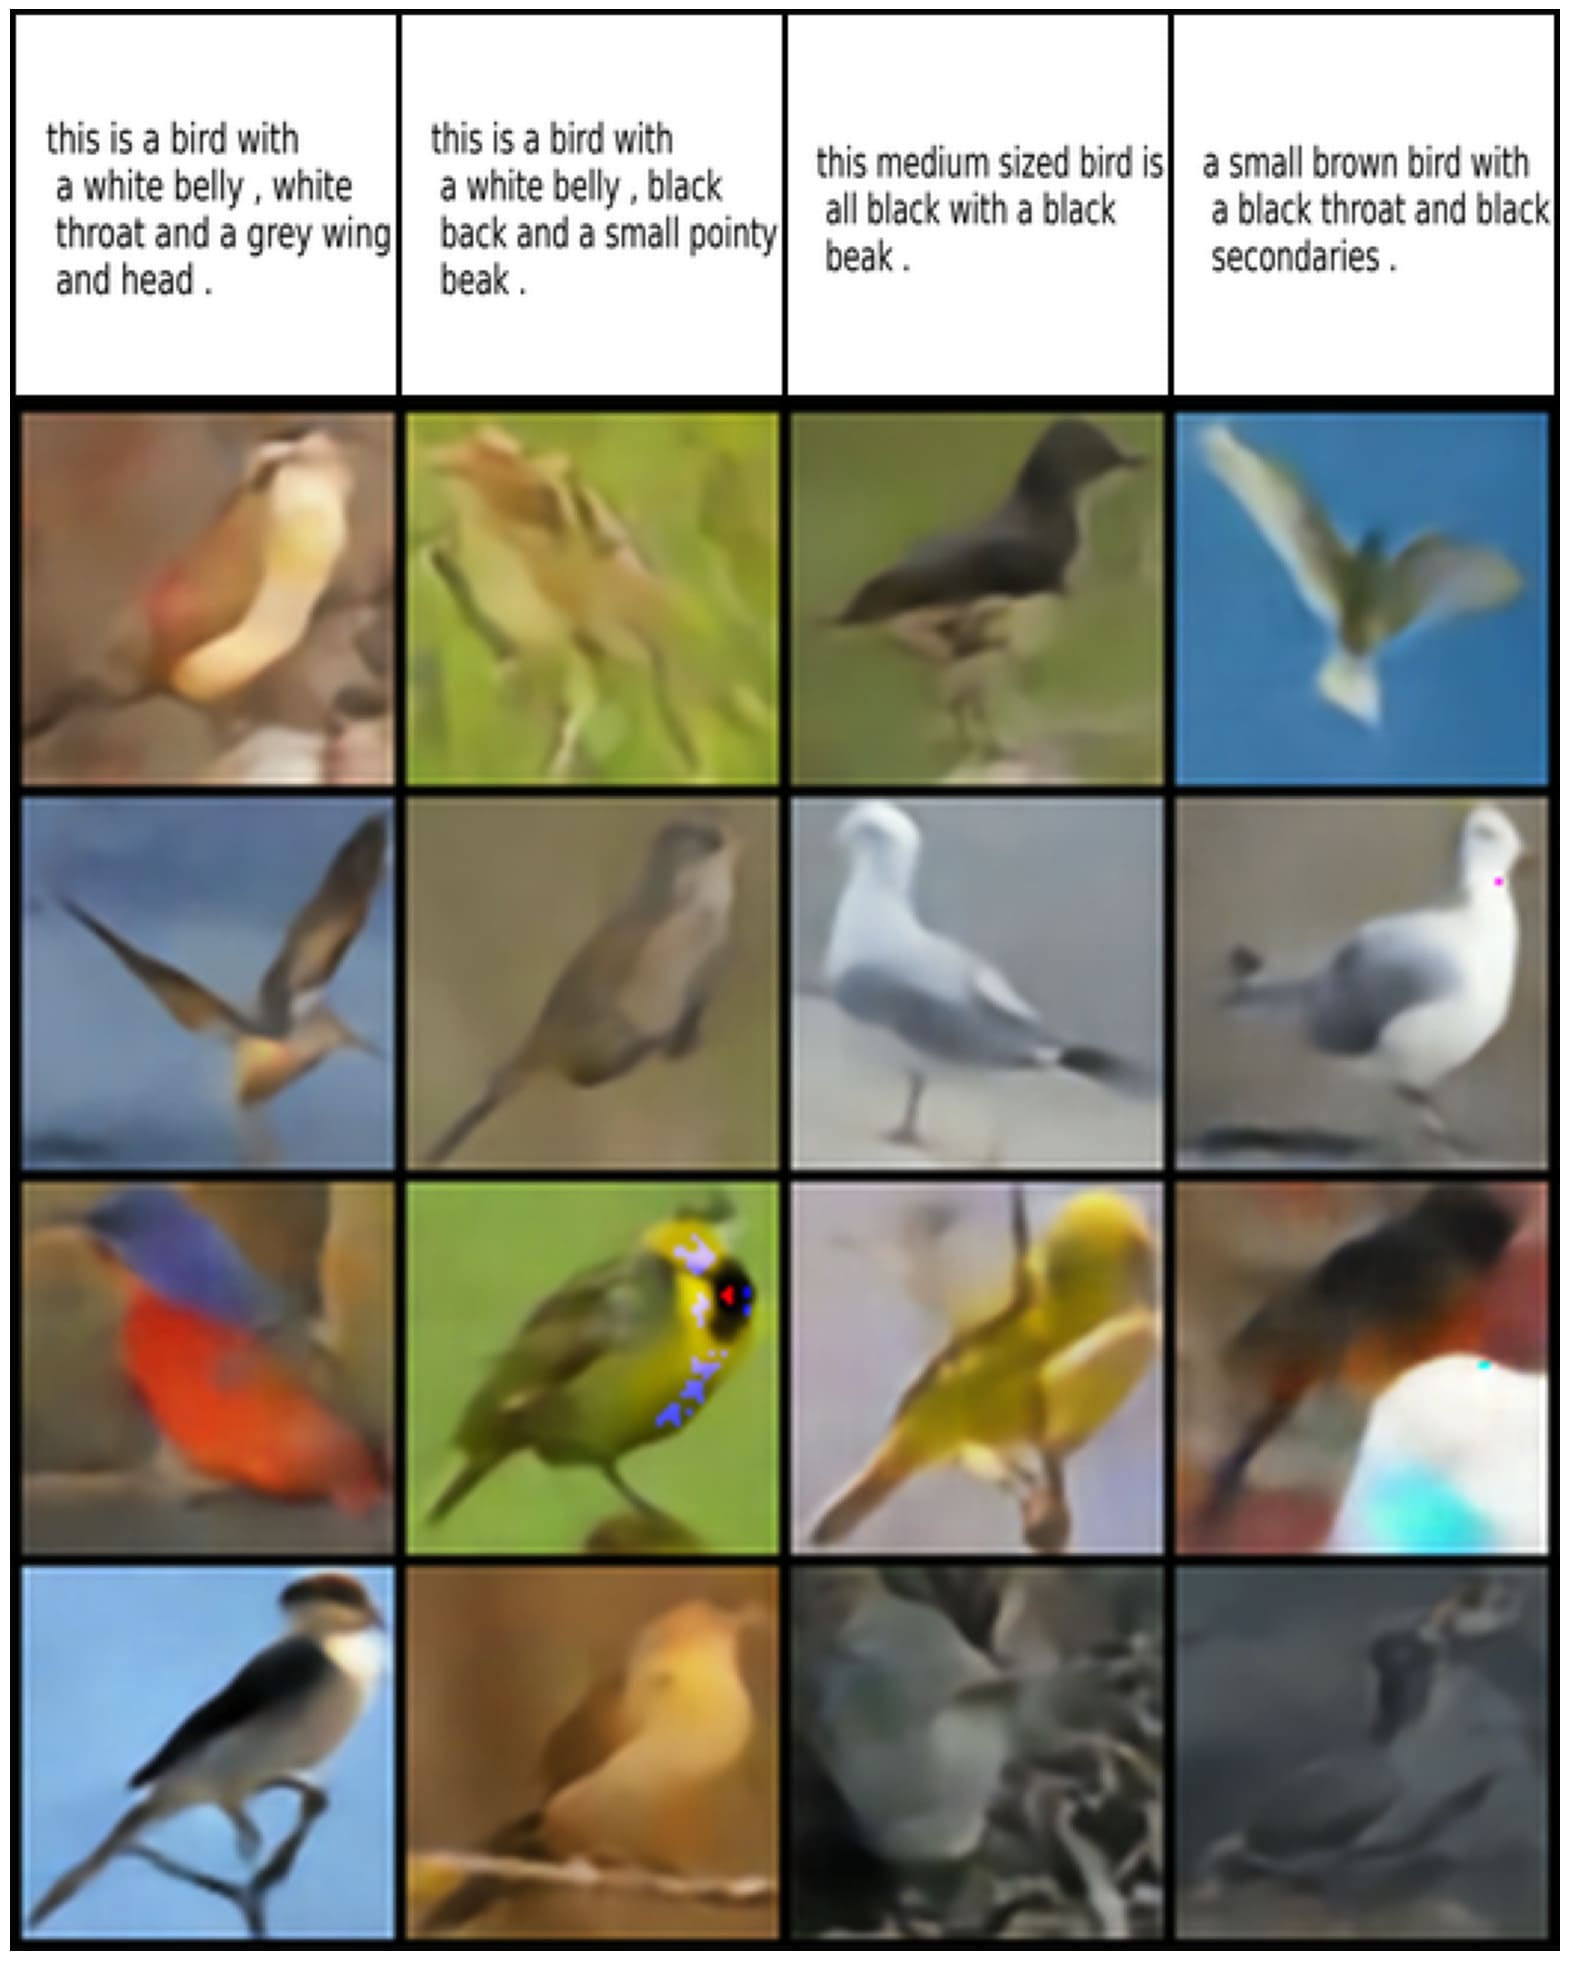
\includegraphics[page=1,width=\linewidth]{figures/datasets/cub/MLD_cond_text_image_mld_var}
         \caption*{\textbf{\gls{MLD} }}
   \end{subfigure}


        \caption{Qualitative results on \textbf{\cub} data-set.
        Caption used as condition to generate the bird images.}
       \label{cap_image_cub_mld}
        
\end{figure}




\subsection{Randomization $d$-ablations study}

The $d$ parameter controls the randomization of the \textit{multi-time masked diffusion process} during training in \Cref{algo:MLD_training}. With probability $d$, the concatenated latent space corresponding to all the modalities is diffused at the same time. With probability $(1-d)$, a portion of the latent space corresponding to a random subset of the modalities is not diffused and freezed during the training step.
To study the parameter $d$ and its effect on the performance of our \gls{MLD} model, we use $d \in \{0.1, .., 0.9\} $.
\Cref{fig:ablationd} shows the $d$-ablations study results on the \textbf{\mnist-\svhn} dataset. 
 We report the performance results averaged over 5 independent seeds as a function of the probability ($1-d$) :
        \textbf{Left:} the conditional and joint coherence for \textbf{\mnist-\svhn} dataset.
        \textbf{Middle:} the quality performance in terms of \gls{FID} for \svhn generation.
         \textbf{Right:} the quality performance in terms of \gls{FMD} for \mnist generation.

We observe that higher value for $1-d$ thus greater probability of applying the \textit{multi-time masked diffusion}, improves the \svhn to \mnist conditional generation coherence. This confirms that the masked multi-time  training enables better conditional generation. Overall, on the \textbf{\mnist-\svhn} dataset, \gls{MLD} shows weak sensibility to the $d$ parameter whenever the value of $d \in [0.2,0.7]$. 

\begin{figure}[H]
     \centering
         \begin{subfigure}[b]{0.28\textwidth}
         \centering
         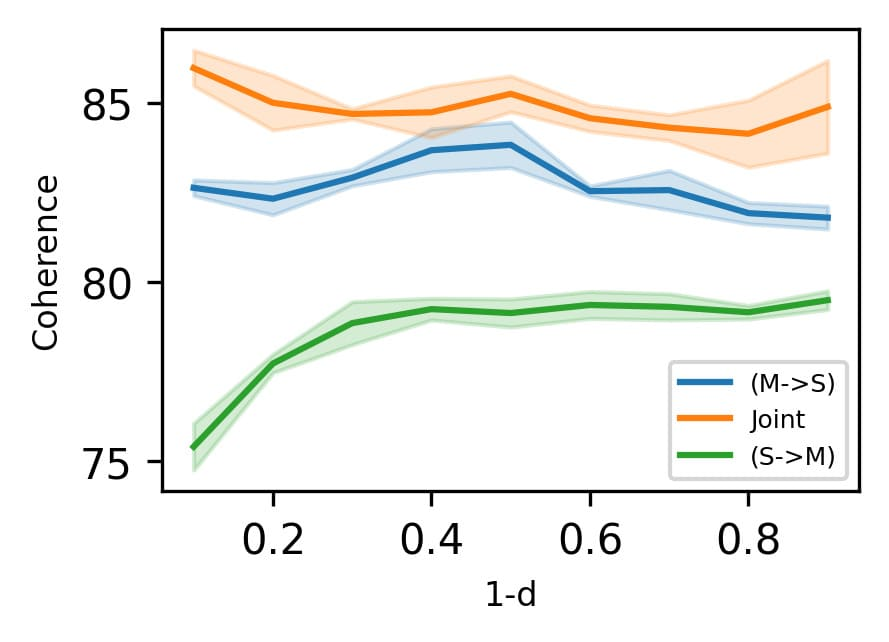
\includegraphics[page=1,width=\linewidth]{figures/datasets/ms/ms_ablation_d_coh}
            \caption{\mnist-\svhn: Coherence (\%$\uparrow$)}
     \end{subfigure}
    \begin{subfigure}[b]{0.28\textwidth}
         \centering
    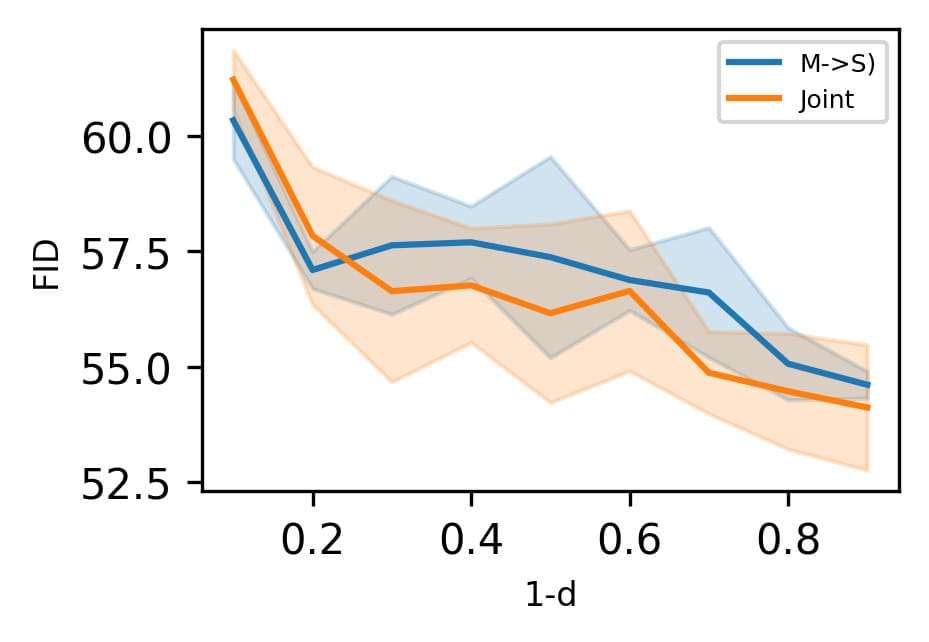
\includegraphics[page=1,width=\linewidth]{figures/datasets/ms/ms_ablation_d_qua_svhn}
           \caption{\svhn:\gls{FID} ($\downarrow$)}
     \end{subfigure}
     \begin{subfigure}{0.28\textwidth}
         \centering
         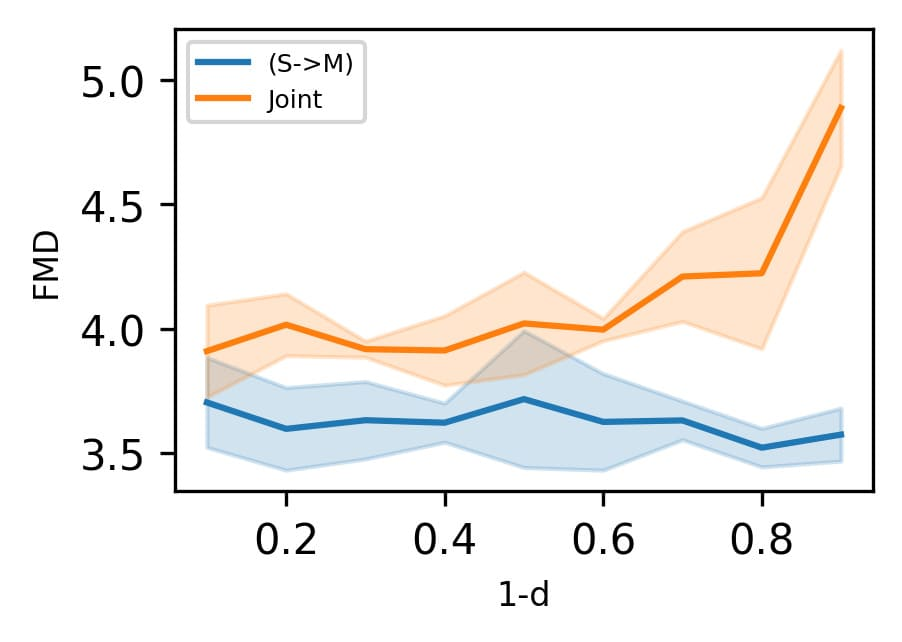
\includegraphics[page=1,width=\linewidth]{figures/datasets/ms/ms_ablation_d_qua_mnist}
            \caption{\mnist:\gls{FMD}($\downarrow$)}
     \end{subfigure}
    \caption{The randomization parameter $d$ ablations study on \textbf{\mnist-\svhn}. }
        \label{fig:ablationd}
\end{figure}


